\documentclass[12pt,openany]{book}
\usepackage[utf8]{inputenc}

% Preamble with packages, custom commands, etc.
\usepackage{commath, amsmath, amsthm}
\usepackage{polynomial}
\usepackage{enumerate}
\usepackage{soul} % highlight
\usepackage{lipsum}  % Just for generating text
\usepackage{etoolbox}

\usepackage{adjustbox}

% Theorem
\newtheorem{axiom}{Axiom}[chapter]
\newtheorem{theorem}{Theorem}[chapter]
\newtheorem{proposition}[theorem]{Proposition}
\newtheorem{corollary}{Corollary}[theorem]
\newtheorem{lemma}[theorem]{Lemma}

\theoremstyle{definition}
\newtheorem{definition}{Definition}[chapter]
\newtheorem{remark}{Remark}[chapter]
\newtheorem{exercise}{Exercise}[chapter]
\newtheorem{example}{Example}[chapter]
\newtheorem*{note}{Note}

% Colors
\usepackage[dvipsnames,table]{xcolor}
\definecolor{titleblue}{RGB}{0,53,128}
\definecolor{chaptergray}{RGB}{140,140,140}
\definecolor{sectiongray}{RGB}{180,180,180}

\definecolor{thmcolor}{RGB}{231, 76, 60}
\definecolor{defcolor}{RGB}{52, 152, 219}
\definecolor{lemcolor}{RGB}{155, 89, 182}
\definecolor{corcolor}{RGB}{46, 204, 113}
\definecolor{procolor}{RGB}{241, 196, 15}
\definecolor{execolor}{RGB}{90, 128, 127}

\definecolor{comments}{HTML}{6A9955} % A kind of forest green.
\definecolor{keyword}{HTML}{569CD6} % A medium blue..
\definecolor{string}{HTML}{CE9178} % A reddish-brown or terra cotta.
\definecolor{function}{HTML}{DCDCAA} % A beige or light khaki.
\definecolor{number}{HTML}{B5CEA8} % A muted green.
\definecolor{type}{HTML}{4EC9B0} %  A turquoise or teal.
\definecolor{class}{HTML}{4EC9B0} % Similar to types, a turquoise or teal.

\definecolor{aesblue}{RGB}{30,144,255}
\definecolor{aesgreen}{RGB}{0,128,0}
\definecolor{aesred}{RGB}{255,69,0}
\definecolor{aesgray}{RGB}{112,128,144}

% Fonts
\usepackage[T1]{fontenc}
\usepackage[utf8]{inputenc}
\usepackage{newpxtext,newpxmath}
\usepackage{sectsty}
\allsectionsfont{\sffamily\color{titleblue}\mdseries}

% Page layout
\usepackage{geometry}
\geometry{a4paper,left=.8in,right=.6in,top=.75in,bottom=1in,heightrounded}
\usepackage{fancyhdr}
\fancyhf{}
\fancyhead[LE,RO]{\thepage}
\fancyhead[LO]{\nouppercase{\rightmark}}
\fancyhead[RE]{\nouppercase{\leftmark}}
\renewcommand{\headrulewidth}{0.5pt}
\renewcommand{\footrulewidth}{0pt}

% Chapter formatting
\usepackage{titlesec}
\titleformat{\chapter}[display]
{\normalfont\sffamily\Huge\bfseries\color{titleblue}}{\chaptertitlename\ \thechapter}{20pt}{\Huge}
\titleformat{\section}
{\normalfont\sffamily\Large\bfseries\color{titleblue!100!gray}}{\thesection}{1em}{}
\titleformat{\subsection}
{\normalfont\sffamily\large\bfseries\color{titleblue!75!gray}}{\thesubsection}{1em}{}

% Table of contents formatting
\usepackage{tocloft}
\renewcommand{\cftchapfont}{\sffamily\color{titleblue}\bfseries}
\renewcommand{\cftsecfont}{\sffamily\color{chaptergray}}
\renewcommand{\cftsubsecfont}{\sffamily\color{sectiongray}}
\renewcommand{\cftchapleader}{\cftdotfill{\cftdotsep}}

% TikZ
\usepackage{tikz}
\usetikzlibrary{matrix, positioning, arrows.meta, calc, shapes.geometric, shapes.multipart, chains}
\usetikzlibrary{decorations.pathreplacing,calligraphy}

% Pseudo-code
\usepackage[linesnumbered,ruled]{algorithm2e}
\usepackage{algpseudocode}
\usepackage{setspace}
\SetKwComment{Comment}{/* }{ */}
\SetKwProg{Fn}{Function}{:}{end}
\SetKwProg{Procedure}{Procedure}{:}{end}
\SetKw{End}{end}
\SetKw{DownTo}{downto}

% Define a new environment for algorithms without line numbers
\newenvironment{algorithm2}[1][]{
	% Save the current state of the algorithm counter
	\newcounter{tempCounter}
	\setcounter{tempCounter}{\value{algocf}}
	% Redefine the algorithm numbering (remove prefix)
	\renewcommand{\thealgocf}{}
	\begin{algorithm}
	}{
	\end{algorithm}
	% Restore the algorithm counter state
	\setcounter{algocf}{\value{tempCounter}}
}


% Listings
\usepackage{listings}
\renewcommand{\lstlistingname}{Code}%
\lstdefinestyle{C}{
	language=C,
	backgroundcolor=\color{white},
	basicstyle=\ttfamily\color{black},
	commentstyle=\color{green!70!black},
	keywordstyle={\bfseries\color{purple}},
	keywordstyle=[2]{\bfseries\color{red}},
	keywordstyle=[3]{\bfseries\color{type}},
	keywordstyle=[4]{\bfseries\color{JungleGreen}},
	keywordstyle=[5]{\bfseries\color{Magenta}},
	keywordstyle=[6]{\bfseries\color{RoyalBlue}},
	keywordstyle=[7]{\bfseries\color{Turquoise}},
	otherkeywords={bool, inline},
	morekeywords=[2]{;},
	morekeywords=[3]{u8,u32,u64,i8,i32,i64},
	morekeywords=[4]{
		rCon, SubWord, RotWord, MUL\_GF256
	},
	morekeywords=[5]{
		KeyExpansion, AddRoundKey,
		SubBytes, InvSubBytes,
		ShiftRows, InvShiftRows,
		MixColumns, InvMixColumns,
		SubMix, InvSubInvMix,
		AES\_Encrypt, AES\_Decrypt
	},
	morekeywords=[6]{false, true, MAX, MIN, GETU32, PUTU32},
	morekeywords=[7]{AES\_VERSION, AES\_BLOCK\_SIZE, ROUND\_KEYS\_SIZE,
		s\_box, inv\_s\_box, Nk, Nr,
		Te0, Te1, Te2, Te3,
		Td0, Td1, Td2, Td3
	},
	numberstyle=\tiny\color{gray},
	stringstyle=\color{purple},
	showstringspaces=false,
	breaklines=true,
	frame=single,
	framesep=3pt,
	%frameround=tttt,
	framexleftmargin=3pt,
	numbers=left,
	numberstyle=\small\color{gray},
	xleftmargin=15pt, % Increase the left margin
	xrightmargin=5pt,
	tabsize=4,
	belowskip=0pt,
	aboveskip=4pt
}
\lstdefinestyle{Rust}{
	language=C, % Set the language to Rust
	backgroundcolor=\color{white},
	basicstyle=\ttfamily\color{black},
	commentstyle=\color{green!70!black},
	keywordstyle={\bfseries\color{purple}},
	keywordstyle=[2]{\bfseries\color{red}},
	keywordstyle=[3]{\bfseries\color{type}},
	keywordstyle=[4]{\bfseries\color{JungleGreen}},
	keywordstyle=[5]{\bfseries\color{Magenta}},
	keywordstyle=[6]{\bfseries\color{RoyalBlue}},
	keywordstyle=[7]{\bfseries\color{Turquoise}},
	otherkeywords={let, mut, fn, impl, trait, enum, struct, match, use, pub, crate, mod},
	morekeywords=[2]{::, ->, =>, |},
	morekeywords=[3]{i8, i32, i64, u8, u32, u64, f32, f64, usize, isize, bool, String, Vec},
	morekeywords=[4]{
		Option, Result, Box, Rc, Arc, Cell, RefCell,
		Thread, Mutex, RwLock, Condvar, Barrier
	},
	morekeywords=[5]{
		println!, format!, vec!, assert!, panic!, unwrap,
		expect, match, if, else, while, for, loop
	},
	alsoletter={!}, % Treat '!' as part of a keyword
	morekeywords=[6]{true, false, Some, None, Ok, Err},
	morekeywords=[7]{std, core, alloc, proc\_macro, test, derive},
	numberstyle=\tiny\color{gray},
	stringstyle=\color{purple},
	showstringspaces=false,
	breaklines=true,
	frame=single,
	framesep=3pt,
	framexleftmargin=3pt,
	numbers=left,
	numberstyle=\small\color{gray},
	xleftmargin=15pt, % Increase the left margin
	xrightmargin=5pt,
	tabsize=4,
	belowskip=0pt,
	aboveskip=4pt
}

\lstdefinestyle{zsh}{
%	language=bash,                  % Set the language to bash (closest to Zsh)
	backgroundcolor=\color{black},
	commentstyle=\color{commentColor}\ttfamily,
	keywordstyle=\color{cyan}\bfseries,
	stringstyle=\color{stringColor}\ttfamily,
	showspaces=false,               % Don't show spaces as underscores
	showstringspaces=false,         % Don't highlight spaces in strings
	breaklines=true,                % Automatic line breaking
	frame=none,                     % No frame around the code
	basicstyle=\ttfamily\color{white}, % White basic text color for contrast
	extendedchars=true,             % Allow extended characters
	captionpos=b,                   % Caption-position at bottom
	escapeinside={\%*}{*)},         % Allow LaTeX inside your code
	morekeywords={echo,ls,pwd,exit,clear,man,unalias,zsh,source}, % Add more keywords
	upquote=true,                   % Ensure straight quotes are used
	literate={\$}{{\textcolor{red}{\$}}}1
	{:}{{\textcolor{red}{:}}}1
	{~}{{\textcolor{red}{\textasciitilde}}}1, % Color certain characters
}

% Table
\usepackage{booktabs}
\usepackage{tabularx}
\usepackage{multicol}
\usepackage{multirow}
\usepackage{array}
\usepackage{longtable}

% Hyperlinks
\usepackage{hyperref}
\hypersetup{
	colorlinks=true,
	linkcolor=titleblue,
	filecolor=black,      
	urlcolor=titleblue,
}

\newcommand{\mathcolorbox}[2]{\colorbox{#1}{$\displaystyle #2$}}
\newcommand{\sol}{\textcolor{magenta}{\bf Sol}}

\newcommand{\F}{\mathbb{F}}
\newcommand{\zero}{\textcolor{red}{\texttt{0}}}
\newcommand{\one}{\textcolor{red}{\texttt{1}}}
\newcommand{\binaryfield}{\set{\zero,\one}}

\newcommand{\ECB}{\mathsf{ECB}}
\newcommand{\CBC}{\mathsf{CBC}}
\newcommand{\OFB}{\mathsf{OFB}}
\newcommand{\CFB}{\mathsf{CFB}}
\newcommand{\CTR}{\mathsf{CTR}}
\newcommand{\CBCCS}{\mathsf{CBC}-\mathsf{CS}}
\newcommand{\EncryptBlk}{\mathsf{EncryptBlk}}
\newcommand{\DecryptBlk}{\mathsf{DecryptBlk}}

\newcommand{\ie}{\textnormal{i.e.}}

\newcommand{\yes}{\textcolor{blue}{O}}
\newcommand{\no}{\textcolor{red}{X}}
\newcommand{\gen}[1]{\langle #1 \rangle}
\newcommand{\Gen}[1]{\left\langle #1 \right\rangle}

\newcommand{\xtime}[1]{\texttt{xtime}\left(#1\right)}
\newcommand{\GF}{\normalfont\text{GF}}

\begin{document}	
	% Title page
	\begin{titlepage}
		\begin{center}
			{\Huge\textsf{\textbf{C | SecureAES}}\par}
			{\Large\textsf{\textbf{- High-Performance AES Encryption in C -}}\par}
			\vspace{0.5in}
			{\Large {Ji Yong-Hyeon}\par}
			\vspace{1in}
%			\begin{center}
%			\begin{tikzpicture}[
%				node distance=1.5cm,
%				auto,
%				block/.style={
%					rectangle, 
%					rounded corners, 
%					draw, 
%					fill=aesblue!30,
%					text width=5em, 
%					text centered, 
%					minimum height=3em
%				},
%				line/.style={
%					draw, 
%					-Latex, 
%					thick
%				},
%				decoration={brace,amplitude=5pt}
%				]
%				
%				% Blocks
%				\node [block] (plaintext) {Plaintext};
%				\node [block, below of=plaintext, fill=aesgreen!30] (key) {Key Expansion};
%				\node [block, below of=key, fill=aesred!30] (subbytes) {SubBytes};
%				\node [block, below of=subbytes, fill=aesgray!30] (shiftrows) {ShiftRows};
%				\node [block, below of=shiftrows, fill=aesblue!30] (mixcolumns) {MixColumns};
%				\node [block, below of=mixcolumns, fill=aesgreen!30] (addroundkey) {AddRoundKey};
%				\node [block, below of=addroundkey] (ciphertext) {Ciphertext};
%				
%				% Arrows
%				\draw [line] (plaintext) -- (key);
%				\draw [line] (key) -- (subbytes);
%				\draw [line] (subbytes) -- (shiftrows);
%				\draw [line] (shiftrows) -- (mixcolumns);
%				\draw [line] (mixcolumns) -- (addroundkey);
%				\draw [line] (addroundkey) -- (ciphertext);
%				
%				% Brace and annotation
%				\draw [decorate, decoration={calligraphic brace, mirror, amplitude=10pt}, thick, aesred] 
%				(subbytes.south west) -- (addroundkey.north west)
%				node[midway, left=10pt, align=left] {Rounds\\Repeated};
%				
%			\end{tikzpicture}
%			\end{center}
			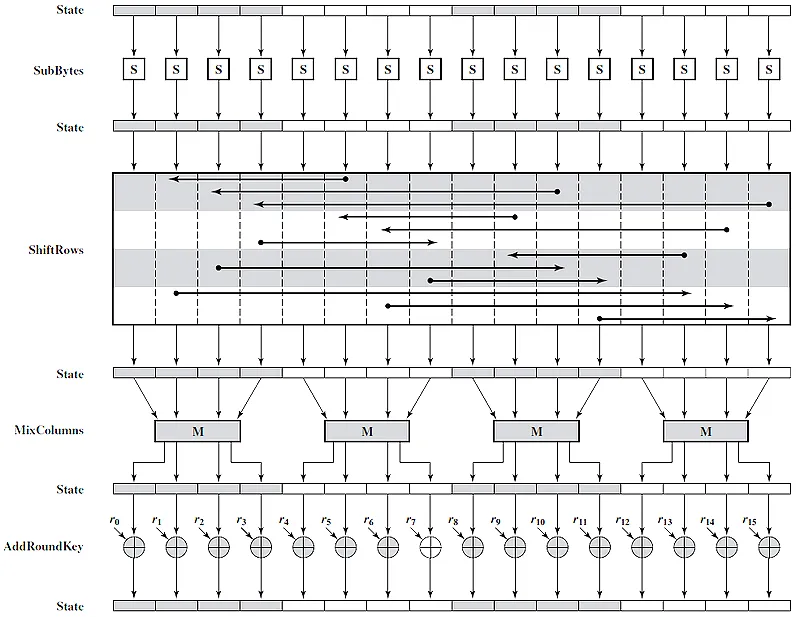
\includegraphics[scale=.6]{images/AES_Encryption_Round.png}\par
			\vspace{1in}
			{\large\bf \textsf{Department of Information Security, Cryptology, and Mathematics}\par}
			{\textsf{College of Science and Technology}\par}
			{\textsf{Kookmin University}\par}
			\vspace{.25in}
			{\large \textsf{\today}\par}
		\end{center}
	\end{titlepage}
	
%	\frontmatter
%	\section*{Acknowledgements}

\begin{note}[\textbf{XOR Operation and Modular Reduction in \( GF(2^n) \)}]
	In the context of Galois Field \( GF(2^n) \), particularly in binary polynomial arithmetic, the XOR operation is equivalent to addition and also plays a crucial role in modular reduction. We explore this equivalence through the principles of field theory and polynomial arithmetic.
	\begin{itemize}
		\item \textbf{Field Properties:}
		
		A Galois Field, \( GF(p^n) \), is a finite field that contains a finite number of elements, where
		\begin{itemize}
			\item \( p \) is a prime number (base of the field) and
			\item \( n \) is a positive integer (degree of the field).
		\end{itemize}
		For the binary field \( GF(2^n) \), \( p = 2 \), which implies that every element in this field is either 0 or 1.
		\vspace{8pt}
		\item \textbf{Addition in \( GF(2^n) \):}
		
		In \( GF(2^n) \), the addition of two elements is performed modulo 2. For any two elements \( a, b \in GF(2^n) \), the addition is defined as:
		\[ a + b = a \oplus b\]
		Since \( 2 \) is the base of the field, the addition wraps around upon reaching 2, which is effectively what the XOR operation does.
		\vspace{8pt}
		\item \textbf{Polynomial Representation:}
		
		Elements in \( GF(2^n) \) can be represented as polynomials where each coefficient is in \( GF(2)=\set{0,1} \). A general element can be written as:
		\[ a(x) = a_{n-1}x^{n-1} + a_{n-2}x^{n-2} + \cdots + a_1x + a_0 \]
		where \( a_i \in \{0, 1\} \) for all \( i \).
		\vspace{8pt}
		\item \textbf{Modular Reduction:}
		
		Modular reduction in \( GF(2^n) \) involves reducing a polynomial by a fixed irreducible polynomial of degree \( n \), ensuring that the result remains within the field. Let \( m(x) \) be the irreducible polynomial. The reduction of a polynomial \( f(x) \) is given by:
		$ f(x) \mod m(x)$
		\vspace{8pt}
		\item \textbf{XOR as Modular Reduction:}
		
		During modular reduction, the subtraction used in polynomial division becomes XOR, because subtraction and addition are the same in \( GF(2) \). Therefore, reducing a polynomial \( f(x) \) by \( m(x) \) is effectively performed using XOR on the coefficients of corresponding terms.
		
		For example, if \( f(x) \) has a term \( x^k \) where \( k \geq n \), and \( m(x) \) has a term \( x^k \), then reducing \( f(x) \) by \( m(x) \) involves XORing the coefficients of \( x^k \) in \( f(x) \) and \( m(x) \), effectively eliminating the \( x^k \) term in \( f(x) \).
	\end{itemize}
	
	In summary, the XOR operation becomes equivalent to both addition and modular reduction in \( GF(2^n) \) due to the binary nature of the field. This equivalence simplifies polynomial arithmetic in binary fields, making it a cornerstone of operations in cryptographic algorithms.
\end{note}

%\section*{Functional Programming}
%
%Functional programming is a paradigm based on mathematical functions, emphasizing expressions and declarations over statements. Key characteristics include:
%
%\begin{itemize}
%	\item \textbf{Immutability}: Data is immutable, which leads to fewer side effects and more predictable code.
%	\item \textbf{First-Class and Higher-Order Functions}: Functions are treated as first-class citizens, allowing them to be passed around, returned, and assigned to variables.
%	\item \textbf{Statelessness}: It avoids shared state and relies on immutable data and pure functions.
%	\item \textbf{Examples}: Haskell, Clojure, and parts of JavaScript, Python, and Scala.
%\end{itemize}
%
%\section*{Imperative Programming}
%
%Imperative programming focuses on a sequence of commands for the computer to perform. Its main features include:
%
%\begin{itemize}
%	\item \textbf{State and Mutability}: Variables in imperative programming can be changed, leading to mutable program states.
%	\item \textbf{Commands and Control Structures}: It utilizes loops, conditionals, and instructions for flow control.
%	\item \textbf{Direct Manipulation of Memory or State}: Often involves changing the program’s state or memory directly.
%	\item \textbf{Examples}: C, C++, Java, and Python.
%\end{itemize}
%
%\section*{Key Differences}
%
%The fundamental distinctions between functional and imperative programming lie in:
%
%\begin{itemize}
%	\item \textbf{Approach to State and Data}: Functional programming uses immutable data, contrasting with the mutable data in imperative programming.
%	\item \textbf{Flow Control}: Function calls and recursion are primary in functional programming, whereas loops and control structures are used in imperative programming.
%	\item \textbf{Side Effects}: Functional programming minimizes side effects, a contrast to the often side-effect-laden imperative programming.
%	\item \textbf{Conciseness and Expressiveness}: Functional programming can be more concise for tasks involving data transformations or concurrent processing.
%	\item \textbf{Learning Curve}: Functional programming often requires a different mindset, focusing on what to solve rather than how, and can have a steeper learning curve.
%\end{itemize}
%
%In contemporary software development, many languages blend elements from both paradigms, offering flexibility and choice to the programmer.
%	\section*{Abstract}

This book is about...

% Your abstract here

	
%	\newpage
%	\tableofcontents
	
	\newpage
	\mainmatter
	\chapter{Block Cipher}
Block ciphers are a fundamental component in cryptographic systems. They transform fixed-size blocks of plaintext into ciphertext using a symmetric key. The transformation is designed to be reversible only with knowledge of the key.

\section{Definition and Structure}

\begin{itemize}
	\item \textbf{Secure Pseudo-Random Permutation (PRP) and Substitution Groups:}
	\begin{itemize}
		\item \textbf{Definition:} A block cipher is considered a secure PRP if it is indistinguishable from a random permutation of the input bits, making it resistant to cryptanalysis.
		\item \textbf{Substitution Groups:} Block ciphers often use substitution-permutation networks (SPNs) that include substitution groups. These groups perform non-linear transformations, crucial for creating cryptographic strength.
	\end{itemize}
	\item \textbf{Confidentiality for Fixed n-bit Data (Blocks):} 
	\begin{itemize}
		\item \textbf{Fixed Block Size:} Block ciphers encrypt and decrypt data in fixed-size blocks (commonly 64 or 128 bits). This fixed size is crucial for the algorithm's structure and security.
		\item \textbf{Padding Schemes:} When the data doesn't fit perfectly into a block, padding schemes are used to fill the remaining space, ensuring consistent block sizes.
	\end{itemize}
	\item \textbf{Block Cipher Operation Modes for Variable-Length Data:} 
	\begin{itemize}
		\item \textbf{Mode of Operation:} To handle variable-length data, block ciphers use different modes of operation like CBC (Cipher Block Chaining), CFB (Cipher Feedback), and GCM (Galois/Counter Mode).
		\item \textbf{Ensuring Security:} Each mode offers distinct features for security and efficiency, often enhancing the cipher's resistance to various attack vectors.
	\end{itemize}
	\item \textbf{Advantages Over Asymmetric Key Cryptography:}
	\begin{itemize}
		\item \textbf{High-Speed Computation:} Block ciphers are generally faster and require less computational power compared to asymmetric key cryptography.
		\item \textbf{Suitability:} This makes them suitable for encrypting large volumes of data and in environments with limited resources.
	\end{itemize}
	\item \textbf{Deriving Other Cryptographic Functions:}
	\begin{itemize}
		\item \textbf{Versatility:} Block ciphers can be used to design other cryptographic functions like hash functions, message authentication codes (MACs), and random number generators.
		\item \textbf{Construction Techniques:} Techniques like Cipher Block Chaining-MAC (CBC-MAC) and Counter mode (CTR) are examples of how block ciphers can be adapted for these purposes.
	\end{itemize}
\end{itemize}

Block ciphers are a critical element in the cryptographic landscape, providing a versatile and efficient means for securing digital data. Their adaptability and robustness make them an indispensable tool in the design of secure communication protocols and cryptographic systems.


\section{Modes of Operations}

\begin{table}[h!]\centering\renewcommand{\arraystretch}{1.05} % Increase row height by 1.5 times
	\caption{Comparison of Modes}
	\begin{tabular*}{\textwidth}{@{\extracolsep{\fill}}cccccccc}
		\toprule[1.2pt]
		Mode & Integrity & Authentication & $\EncryptBlk$ & $\DecryptBlk$ & Padding & IV & $\abs{P}\overset{?}{=}\abs{C}$ \\
		\midrule
		$\ECB$ & \yes & \no & \yes & \yes & \yes & \no & $\abs{P}<\abs{C}$ \\
		$\CBC$ & \yes & \no & \yes & \yes & \yes & \yes & $\abs{P}<\abs{C}$ \\
		$\OFB$ & \yes & \no & \yes & \no & \no & \yes & $\abs{P}=\abs{C}$ \\
		$\CFB$ & \yes & \no & \yes & \no & \no & \yes & $\abs{P}=\abs{C}$ \\
		$\CTR$ & \yes & \no & \yes & \no & \no & \yes & $\abs{P}=\abs{C}$ \\
		$\CBCCS$ & \yes & \no & \yes & \yes & \no & \yes & $\abs{P}=\abs{C}$ \\
		\bottomrule[1.2pt]
	\end{tabular*}
\end{table}

\subsection{Padding}
Block ciphers require input lengths to be a multiple of the block size. Padding is used to extend the last block of plaintext to the required length. Without proper padding, the encryption process may be insecure or infeasible.\\
\\
There are several padding schemes used in practice, such as:
\begin{table}[ht]
	\centering\renewcommand{\arraystretch}{1.05}
	\caption{Padding Standards in Block Ciphers}
	\begin{tabular*}{\textwidth}{>{\bfseries}l l}
		\toprule
		\textbf{Standard Name} & \textbf{Padding Method} \\
		\midrule
		\multirow{2}{*}{PKCS\#7} & Pad with bytes all the same value as the number of padding bytes \\
		& \texttt{\dots dd | dd dd dd dd dd dd dd dd dd dd dd dd \textcolor{red}{04} \textcolor{red}{04} \textcolor{red}{04} \textcolor{red}{04}} | \\
		\hline
		\multirow{2}{*}{ANSI X9.23} & Pad with zeros, last byte is the number of padding bytes \\
		& \texttt{\dots dd | dd dd dd dd dd dd dd dd dd dd dd \textcolor{red}{00} \textcolor{red}{00} \textcolor{red}{00} \textcolor{red}{00} \textcolor{red}{05}} | \\
		\hline
		\multirow{2}{*}{ISO/IEC 7816-4} & First byte is '80' (hex), followed by zeros \\
		& \texttt{\dots dd | dd dd dd dd dd dd dd dd dd dd \textcolor{red}{80} \textcolor{red}{00} \textcolor{red}{00} \textcolor{red}{00} \textcolor{red}{00} \textcolor{red}{00}} | \\
		\hline
		\multirow{2}{*}{ISO 10126} & Pad with random bytes, last byte is the number of padding bytes \\
		& \texttt{\dots dd | dd dd dd dd dd dd dd dd dd dd \textcolor{red}{2e} \textcolor{red}{49} \textcolor{red}{1b} \textcolor{red}{c1} \textcolor{red}{aa} \textcolor{red}{06}} | \\
		\bottomrule
	\end{tabular*}
	\label{tab:padding_standards}
\end{table}

\newpage

\subsection{$\ECB$ (Electronic CodeBook)}
\begin{algorithm}[H]
	\caption{Electronic CodeBook}
	\begin{multicols}{2}
		\KwIn{$K$ and $P=P_1\parallel\cdots\parallel P_N$ ($P_i\in\binaryfield^{n}$)}
		\KwOut{$C=C_1\parallel\cdots\parallel C_N$ ($C_i\in\binaryfield^n$)}
		\BlankLine
		\For{$i\gets 1$ \KwTo $N$}{
			$C_i\gets\EncryptBlk(K, P_i)$\;
		}
		\Return $C=C_1\parallel\cdots\parallel C_N$\;
		\columnbreak % Move to the next column
		\setcounter{AlgoLine}{0}  % Reset line numbering
		\KwIn{$K$ and $C=C_1\parallel\cdots\parallel C_N$ ($C_i\in\binaryfield^n$)}
		\KwOut{$P=P_1\parallel\cdots\parallel P_N$ ($P_i\in\binaryfield^{n}$)}
		\BlankLine
		\For{$i\gets 1$ \KwTo $N$}{
			$P_i\gets\DecryptBlk(K, C_i)$\;
		}
		\Return $C=C_1\parallel\cdots\parallel C_N$\;
	\end{multicols}
	\BlankLine
\end{algorithm}
\vspace{12pt}
\begin{center}
\begin{minipage}{.49\textwidth}\centering
\begin{tikzpicture}
	% Define styles
	\tikzset{
		block/.style={rectangle, draw, fill=blue!20, text width=2em, text centered, minimum height=2.5em},
		line/.style={draw, -Latex}
	}
	
	% Nodes
	\node[block] (p1) {$P_1$};
	\node[block, right=of p1] (p2) {$P_2$};
	\node[block, right=of p2] (p3) {...};
	\node[block, right=of p3] (p4) {$P_N$};
	
	\node[block, below=of p1] (e1) {$E_K$};
	\node[block, below=of p2] (e2) {$E_K$};
	\node[block, below=of p3] (e3) {...};
	\node[block, below=of p4] (e4) {$E_K$};
	
	\node[block, below=of e1] (c1) {$C_1$};
	\node[block, below=of e2] (c2) {$C_2$};
	\node[block, below=of e3] (c3) {...};
	\node[block, below=of e4] (c4) {$C_N$};
	
	% Arrows
	\path [line] (p1) -- (e1);
	\path [line] (p2) -- (e2);
	\path [line] (p3) -- (e3);
	\path [line] (p4) -- (e4);
	
	\path [line] (e1) -- (c1);
	\path [line] (e2) -- (c2);
	\path [line] (e3) -- (c3);
	\path [line] (e4) -- (c4);
\end{tikzpicture}
\end{minipage}
\begin{minipage}{.49\textwidth}\centering
\begin{tikzpicture}
	% Define styles
	\tikzset{
		block/.style={rectangle, draw, fill=red!20, text width=2em, text centered, minimum height=2.5em},
		line/.style={draw, -Latex}
	}
	
	% Nodes
	\node[block] (p1) {$P_1$};
	\node[block, right=of p1] (p2) {$P_2$};
	\node[block, right=of p2] (p3) {...};
	\node[block, right=of p3] (p4) {$P_N$};
	
	\node[block, below=of p1] (e1) {$E_K$};
	\node[block, below=of p2] (e2) {$E_K$};
	\node[block, below=of p3] (e3) {...};
	\node[block, below=of p4] (e4) {$E_K$};
	
	\node[block, below=of e1] (c1) {$C_1$};
	\node[block, below=of e2] (c2) {$C_2$};
	\node[block, below=of e3] (c3) {...};
	\node[block, below=of e4] (c4) {$C_N$};
	
	% Arrows
	\path [line] (e1) -- (p1);
	\path [line] (e2) -- (p2);
	\path [line] (e3) -- (p3);
	\path [line] (e4) -- (p4);
	
	\path [line] (c1) -- (e1);
	\path [line] (c2) -- (e2);
	\path [line] (c3) -- (e3);
	\path [line] (c4) -- (e4);
\end{tikzpicture}
\end{minipage}

\end{center}

\vspace{24pt}
\begin{remark}
\ \begin{enumerate}[(1)]
	\item For a pair of plaintext/ciphertext $(P, C)$ and $(P', C')$, \[
	P=P'\implies C=C'.
	\]
	\item A single-bit error in the ciphertext affects only the corresponding block in the decryption.
	\item Block order changes, as well as additions/deletions, are possible. Therefore, to ensure the integrity of the ciphertext (i.e., detection or prevention of tampering), it should be used in conjunction with a checksum or a Message Authentication Code (MAC).
\end{enumerate}
\end{remark}

\newpage
\subsection{$\CBC$ (Cipher Block Chaining)}
\begin{algorithm}[H]
	\caption{Cipher Block Chaining}
	\begin{multicols}{2}
		\KwIn{$K$, $IV$ and $P=P_1\parallel\cdots\parallel P_N$}
		\KwOut{$C=C_1\parallel\cdots\parallel C_N$}
		\BlankLine
		$C_0\gets IV$\;
		\For{$i\gets 1$ \KwTo $N$}{
			$C_i\gets\EncryptBlk(K, P_i\oplus C_{i-1})$\;
		}
		\Return $C=C_1\parallel\cdots\parallel C_N$\;
		\columnbreak % Move to the next column
		\setcounter{AlgoLine}{0}  % Reset line numbering
		\KwIn{$K$, $IV$ and $C=C_1\parallel\cdots\parallel C_N$}
		\KwOut{$P=P_1\parallel\cdots\parallel P_N$}
		\BlankLine
		$C_0\gets IV$\;
		\For{$i\gets 1$ \KwTo $N$}{
			$P_i\gets C_{i-1}\oplus\DecryptBlk(K, C_{i})$\;
		}
		\Return $P=P_1\parallel\cdots\parallel P_N$\;
	\end{multicols}
	\BlankLine
\end{algorithm}

\begin{center}
\begin{minipage}{.49\textwidth}\centering
\begin{tikzpicture}
	% Define styles
	\tikzset{
		block/.style={rectangle, draw, fill=blue!20, text width=1em, text centered, minimum height=1em},
		line/.style={draw, -Latex},
		xor/.style={circle, draw, minimum size=0cm, inner sep=0pt}
	}
	% Nodes
	\node[block] (iv) {IV};
	\node[block, right=1cm of iv] (p1) {$P_1$};
	\node[block, right=1cm of p1] (p2) {$P_2$};
	\node[block, right=1cm of p2] (p3) {...};
	\node[block, right=1cm of p3] (p4) {$P_n$};
	
	\node[below=1cm of p1] (xor1) {\Huge $\oplus$};
	\node[below=1cm of p2] (xor2) {\Huge $\oplus$};
	\node[below=1cm of p3] (xor3) {\Huge $\oplus$};
	\node[below=1cm of p4] (xor4) {\Huge $\oplus$};
	
	\node[block, below=1cm of xor1] (e1) {$E_K$};
	\node[block, below=1cm of xor2] (e2) {$E_K$};
	\node[block, below=1cm of xor3] (e3) {...};
	\node[block, below=1cm of xor4] (e4) {$E_K$};
	
	\node[block, below=1cm of e1] (c1) {$C_1$};
	\node[block, below=1cm of e2] (c2) {$C_2$};
	\node[block, below=1cm of e3] (c3) {...};
	\node[block, below=1cm of e4] (c4) {$C_n$};
	
	% Arrows
	\draw[line] (iv.south) to[bend right=45] (xor1.west);
	\draw[line] (p1) -- (xor1);
	\draw[line] (xor1) -- (e1);
	\draw[line] (e1) -- (c1);
	
	\draw[line] (e1.south) to[bend right=90] ($(c1)!.6!(e2)$) to[bend left=60] (xor2.west);
	\draw[line] (p2) -- (xor2);
	\draw[line] (xor2) -- (e2);
	\draw[line] (e2) -- (c2);
	
	\draw[line] (c2.east) to[bend right=45] ($(c2)!.5!(xor3)$) to[bend left=45] (xor3.west);
	\draw[line] (p3) -- (xor3);
	\draw[line] (xor3) -- (e3);
	\draw[line] (e3) -- (c3);
	
	\draw[line] (c3.east) to[bend right=45] ($(c3)!.5!(xor4)$) to[bend left=45] (xor4.west);
	\draw[line] (p4) -- (xor4);
	\draw[line] (xor4) -- (e4);
	\draw[line] (e4) -- (c4);
\end{tikzpicture}
\end{minipage}
\begin{minipage}{.49\textwidth}\centering
	\begin{tikzpicture}
		% Define styles
		\tikzset{
			block/.style={rectangle, draw, fill=blue!20, text width=1em, text centered, minimum height=1em},
			line/.style={draw, -Latex},
			xor/.style={circle, draw, minimum size=0cm, inner sep=0pt}
		}
		
		% Nodes
		\node[block] (iv) {IV};
		\node[block, right=1cm of iv] (p1) {$P_1$};
		\node[block, right=1cm of p1] (p2) {$P_2$};
		\node[block, right=1cm of p2] (p3) {...};
		\node[block, right=1cm of p3] (p4) {$P_n$};
		
		\node[below=1cm of p1] (xor1) {\Huge $\oplus$};
		\node[below=1cm of p2] (xor2) {\Huge $\oplus$};
		\node[below=1cm of p3] (xor3) {\Huge $\oplus$};
		\node[below=1cm of p4] (xor4) {\Huge $\oplus$};
		
		\node[block, below=1cm of xor1] (e1) {$E_K$};
		\node[block, below=1cm of xor2] (e2) {$E_K$};
		\node[block, below=1cm of xor3] (e3) {...};
		\node[block, below=1cm of xor4] (e4) {$E_K$};
		
		\node[block, below=1cm of e1] (c1) {$C_1$};
		\node[block, below=1cm of e2] (c2) {$C_2$};
		\node[block, below=1cm of e3] (c3) {...};
		\node[block, below=1cm of e4] (c4) {$C_n$};
		
		% Arrows
		\draw[line] (iv.south) to[bend right=45] (xor1.west);
		\draw[line] (xor1) -- (p1);
		\draw[line] (e1) -- (xor1);
		\draw[line] (c1) -- (e1);
		
		\draw[line] (c1.east) to[bend right=45] ($(c1)!.5!(xor2)$) to[bend left=45] (xor2.west);
		\draw[line] (xor2) -- (p2);
		\draw[line] (e2) -- (xor2);
		\draw[line] (c2) -- (e2);
		
		\draw[line] (c2.east) to[bend right=45] ($(c2)!.5!(xor3)$) to[bend left=45] (xor3.west);
		\draw[line] (xor3) -- (p3);
		\draw[line] (e3) -- (xor3);
		\draw[line] (c3) -- (e3);
		
		\draw[line] (c3.east) to[bend right=45] ($(c3)!.5!(xor4)$) to[bend left=45] (xor4.west);
		\draw[line] (xor4) -- (p4);
		\draw[line] (e4) -- (xor4);
		\draw[line] (c4) -- (e4);
	\end{tikzpicture}
\end{minipage}
\end{center}

\vspace{24pt}
\begin{remark}
\ \begin{enumerate}[(1)]
	\item For a set of plaintext/ciphertext pairs $(IV, P, C)$ and $(IV', P', C')$, \[
	IV=IV'\land P=P'\implies C=C'.
	\]
	\item  A one-bit error in the ciphertext will affect the corresponding block and the subsequent block in the decryption process, thereby enabling the detection of such errors.
	\item Altering the order of blocks, as well as adding or deleting them, is not possible.
\end{enumerate}
\end{remark}
\newpage
\subsection{$\OFB$ (Output FeedBack)}
\begin{center}
\begin{tikzpicture}
	% Define styles
	\tikzset{
		block/.style={rectangle, draw, fill=blue!20, text width=2.5em, text centered, minimum height=2.5em},
		line/.style={draw, -Latex},
		xor/.style={circle, draw, minimum size=0.75cm, inner sep=0pt}
	}
	
	% Nodes
	\node[block] (iv) {IV};
	\node[block, right=1cm of iv] (e1) {$E$};
	\node[block, right=1cm of e1] (e2) {$E$};
	\node[block, right=1cm of e2] (e3) {...};
	\node[block, right=1cm of e3] (e4) {$E$};
	
	\node[block, above=1cm of e1] (p1) {P1};
	\node[block, above=1cm of e2] (p2) {P2};
	\node[block, above=1cm of e3] (p3) {...};
	\node[block, above=1cm of e4] (p4) {Pn};
	
	\node[block, below=1cm of e1] (c1) {C1};
	\node[block, below=1cm of e2] (c2) {C2};
	\node[block, below=1cm of e3] (c3) {...};
	\node[block, below=1cm of e4] (c4) {Cn};
	
	\node[xor, right=0.5cm of p1] (xor1) {\large $\oplus$};
	\node[xor, right=0.5cm of p2] (xor2) {\large $\oplus$};
	\node[xor, right=0.5cm of p3] (xor3) {\large $\oplus$};
	\node[xor, right=0.5cm of p4] (xor4) {\large $\oplus$};
	
	% Arrows
	\draw[line] (iv) -- (e1);
	\draw[line] (e1) -- (e2);
	\draw[line] (e2) -- (e3);
	\draw[line] (e3) -- (e4);
	
	\draw[line] (e1) -- (xor1);
	\draw[line] (e2) -- (xor2);
	\draw[line] (e3) -- (xor3);
	\draw[line] (e4) -- (xor4);
	
	\draw[line] (p1) -- (xor1);
	\draw[line] (p2) -- (xor2);
	\draw[line] (p3) -- (xor3);
	\draw[line] (p4) -- (xor4);
	
	\draw[line] (xor1) -- (c1);
	\draw[line] (xor2) -- (c2);
	\draw[line] (xor3) -- (c3);
	\draw[line] (xor4) -- (c4);
	
\end{tikzpicture}
\end{center}

\subsection{$\CFB$ (Ciphertext FeedBack)}
\begin{center}
\begin{tikzpicture}
	% Define styles
	\tikzset{
		block/.style={rectangle, draw, fill=blue!20, text width=2.5em, text centered, minimum height=2.5em},
		line/.style={draw, -Latex},
		xor/.style={circle, draw, minimum size=0.75cm, inner sep=0pt}
	}
	
	% Nodes
	\node[block] (iv) {IV};
	\node[block, right=1cm of iv] (e1) {$E$};
	\node[block, right=1cm of e1] (e2) {$E$};
	\node[block, right=1cm of e2] (e3) {...};
	\node[block, right=1cm of e3] (e4) {$E$};
	
	\node[block, above=1cm of e1] (p1) {P1};
	\node[block, above=1cm of e2] (p2) {P2};
	\node[block, above=1cm of e3] (p3) {...};
	\node[block, above=1cm of e4] (p4) {Pn};
	
	\node[block, below=1cm of e1] (c1) {C1};
	\node[block, below=1cm of e2] (c2) {C2};
	\node[block, below=1cm of e3] (c3) {...};
	\node[block, below=1cm of e4] (c4) {Cn};
	
	\node[xor, right=0.5cm of iv] (xor1) {\large $\oplus$};
	\node[xor, right=0.5cm of e1] (xor2) {\large $\oplus$};
	\node[xor, right=0.5cm of e2] (xor3) {\large $\oplus$};
	\node[xor, right=0.5cm of e3] (xor4) {\large $\oplus$};
	
	% Arrows
	\draw[line] (iv) -- (xor1);
	\draw[line] (xor1) -- (e1);
	\draw[line] (e1) -- (xor2);
	\draw[line] (xor2) -- (e2);
	\draw[line] (e2) -- (xor3);
	\draw[line] (xor3) -- (e3);
	\draw[line] (e3) -- (xor4);
	\draw[line] (xor4) -- (e4);
	
	\draw[line] (p1) -- (xor1);
	\draw[line] (p2) -- (xor2);
	\draw[line] (p3) -- (xor3);
	\draw[line] (p4) -- (xor4);
	
	\draw[line] (e1) -- (c1);
	\draw[line] (e2) -- (c2);
	\draw[line] (e3) -- (c3);
	\draw[line] (e4) -- (c4);
	
\end{tikzpicture}
\end{center}

\subsection{$\CTR$ (CounTeR)}
\begin{center}
\begin{tikzpicture}
	% Define styles
	\tikzset{
		block/.style={rectangle, draw, fill=blue!20, text width=2.5em, text centered, minimum height=2.5em},
		line/.style={draw, -Latex},
		xor/.style={circle, draw, minimum size=0.75cm, inner sep=0pt},
		counter/.style={rectangle, draw, fill=red!20, text width=2.5em, text centered, minimum height=2.5em}
	}
	
	% Nodes
	\node[counter] (iv) {IV};
	\node[block, right=1cm of iv] (e1) {$E$};
	\node[counter, right=1cm of e1] (cnt1) {Cnt+1};
	\node[block, right=1cm of cnt1] (e2) {$E$};
	\node[counter, right=1cm of e2] (cnt2) {Cnt+2};
	\node[block, right=1cm of cnt2] (e3) {...};
	
	\node[block, above=1cm of e1] (p1) {P1};
	\node[block, above=1cm of e2] (p2) {P2};
	\node[block, above=1cm of e3] (p3) {...};
	
	\node[block, below=1cm of e1] (c1) {C1};
	\node[block, below=1cm of e2] (c2) {C2};
	\node[block, below=1cm of e3] (c3) {...};
	
	\node[xor, right=0.5cm of p1] (xor1) {\large $\oplus$};
	\node[xor, right=0.5cm of p2] (xor2) {\large $\oplus$};
	\node[xor, right=0.5cm of p3] (xor3) {\large $\oplus$};
	
	% Arrows
	\draw[line] (iv) -- (e1);
	\draw[line] (cnt1) -- (e2);
	\draw[line] (cnt2) -- (e3);
	
	\draw[line] (e1) -- (xor1);
	\draw[line] (e2) -- (xor2);
	\draw[line] (e3) -- (xor3);
	
	\draw[line] (p1) -- (xor1);
	\draw[line] (p2) -- (xor2);
	\draw[line] (p3) -- (xor3);
	
	\draw[line] (xor1) -- (c1);
	\draw[line] (xor2) -- (c2);
	\draw[line] (xor3) -- (c3);
	
\end{tikzpicture}
\end{center}

\begin{center}



\tikzset{every picture/.style={line width=0.75pt}} %set default line width to 0.75pt        

\begin{tikzpicture}[x=0.75pt,y=0.75pt,yscale=-1,xscale=1]
	%uncomment if require: \path (0,453); %set diagram left start at 0, and has height of 453
	
	\draw   (136,319.33) .. controls (136,311.05) and (142.72,304.33) .. (151,304.33) .. controls (159.28,304.33) and (166,311.05) .. (166,319.33) .. controls (166,327.62) and (159.28,334.33) .. (151,334.33) .. controls (142.72,334.33) and (136,327.62) .. (136,319.33) -- cycle ; \draw   (136,319.33) -- (166,319.33) ; \draw   (151,304.33) -- (151,334.33) ;
	\draw   (336,316) .. controls (336,307.72) and (342.72,301) .. (351,301) .. controls (359.28,301) and (366,307.72) .. (366,316) .. controls (366,324.28) and (359.28,331) .. (351,331) .. controls (342.72,331) and (336,324.28) .. (336,316) -- cycle ; \draw   (336,316) -- (366,316) ; \draw   (351,301) -- (351,331) ;
	\draw   (536.67,320) .. controls (536.67,311.72) and (543.38,305) .. (551.67,305) .. controls (559.95,305) and (566.67,311.72) .. (566.67,320) .. controls (566.67,328.28) and (559.95,335) .. (551.67,335) .. controls (543.38,335) and (536.67,328.28) .. (536.67,320) -- cycle ; \draw   (536.67,320) -- (566.67,320) ; \draw   (551.67,305) -- (551.67,335) ;
	%Shape: Rectangle [id:dp23698905140771065] 
	\draw   (92.5,164.67) -- (209.5,164.67) -- (209.5,236.67) -- (92.5,236.67) -- cycle ;
	%Shape: Rectangle [id:dp060189272097281865] 
	\draw   (292.5,164.67) -- (409.5,164.67) -- (409.5,236.67) -- (292.5,236.67) -- cycle ;
	%Shape: Rectangle [id:dp7358028365384404] 
	\draw   (492.17,164.67) -- (609.17,164.67) -- (609.17,236.67) -- (492.17,236.67) -- cycle ;
	%Straight Lines [id:da6855921879025784] 
	\draw    (150.33,237.33) -- (150.97,300.4) ;
	\draw [shift={(151,303.4)}, rotate = 269.42] [fill={rgb, 255:red, 0; green, 0; blue, 0 }  ][line width=0.08]  [draw opacity=0] (8.93,-4.29) -- (0,0) -- (8.93,4.29) -- cycle    ;
	%Straight Lines [id:da8393200361220992] 
	\draw    (351,237.33) -- (351.64,300.4) ;
	\draw [shift={(351.67,303.4)}, rotate = 269.42] [fill={rgb, 255:red, 0; green, 0; blue, 0 }  ][line width=0.08]  [draw opacity=0] (8.93,-4.29) -- (0,0) -- (8.93,4.29) -- cycle    ;
	%Straight Lines [id:da812579829875762] 
	\draw    (550.67,237.33) -- (551.3,300.4) ;
	\draw [shift={(551.33,303.4)}, rotate = 269.42] [fill={rgb, 255:red, 0; green, 0; blue, 0 }  ][line width=0.08]  [draw opacity=0] (8.93,-4.29) -- (0,0) -- (8.93,4.29) -- cycle    ;
	%Straight Lines [id:da8953409064226481] 
	\draw    (65,320.33) -- (134,320.33) ;
	\draw [shift={(137,320.33)}, rotate = 180] [fill={rgb, 255:red, 0; green, 0; blue, 0 }  ][line width=0.08]  [draw opacity=0] (8.93,-4.29) -- (0,0) -- (8.93,4.29) -- cycle    ;
	%Straight Lines [id:da29517048533379] 
	\draw    (150.33,79.8) -- (150.98,161.67) ;
	\draw [shift={(151,164.67)}, rotate = 269.55] [fill={rgb, 255:red, 0; green, 0; blue, 0 }  ][line width=0.08]  [draw opacity=0] (8.93,-4.29) -- (0,0) -- (8.93,4.29) -- cycle    ;
	%Straight Lines [id:da14835328393275948] 
	\draw    (351,79.8) -- (351.64,161.67) ;
	\draw [shift={(351.67,164.67)}, rotate = 269.55] [fill={rgb, 255:red, 0; green, 0; blue, 0 }  ][line width=0.08]  [draw opacity=0] (8.93,-4.29) -- (0,0) -- (8.93,4.29) -- cycle    ;
	%Straight Lines [id:da5864783489550343] 
	\draw    (550,79.8) -- (550.64,161.67) ;
	\draw [shift={(550.67,164.67)}, rotate = 269.55] [fill={rgb, 255:red, 0; green, 0; blue, 0 }  ][line width=0.08]  [draw opacity=0] (8.93,-4.29) -- (0,0) -- (8.93,4.29) -- cycle    ;
	%Straight Lines [id:da997385537510096] 
	\draw    (150.33,332.67) -- (150.97,395.67) ;
	\draw [shift={(151,398.67)}, rotate = 269.42] [fill={rgb, 255:red, 0; green, 0; blue, 0 }  ][line width=0.08]  [draw opacity=0] (8.93,-4.29) -- (0,0) -- (8.93,4.29) -- cycle    ;
	%Straight Lines [id:da9215134990511367] 
	\draw    (351,332.67) -- (351.64,395.67) ;
	\draw [shift={(351.67,398.67)}, rotate = 269.42] [fill={rgb, 255:red, 0; green, 0; blue, 0 }  ][line width=0.08]  [draw opacity=0] (8.93,-4.29) -- (0,0) -- (8.93,4.29) -- cycle    ;
	%Straight Lines [id:da6364900722654636] 
	\draw    (550.67,332.67) -- (551.3,395.67) ;
	\draw [shift={(551.33,398.67)}, rotate = 269.42] [fill={rgb, 255:red, 0; green, 0; blue, 0 }  ][line width=0.08]  [draw opacity=0] (8.93,-4.29) -- (0,0) -- (8.93,4.29) -- cycle    ;
	%Straight Lines [id:da46397299472270315] 
	\draw    (265,315.33) -- (334,315.33) ;
	\draw [shift={(337,315.33)}, rotate = 180] [fill={rgb, 255:red, 0; green, 0; blue, 0 }  ][line width=0.08]  [draw opacity=0] (8.93,-4.29) -- (0,0) -- (8.93,4.29) -- cycle    ;
	%Straight Lines [id:da48196890203542964] 
	\draw    (465,319.33) -- (534,319.33) ;
	\draw [shift={(537,319.33)}, rotate = 180] [fill={rgb, 255:red, 0; green, 0; blue, 0 }  ][line width=0.08]  [draw opacity=0] (8.93,-4.29) -- (0,0) -- (8.93,4.29) -- cycle    ;
	
	% Text Node
	\draw (133,53.07) node [anchor=north west][inner sep=0.75pt]    {$CTR$};
	% Text Node
	\draw (319.5,53.07) node [anchor=north west][inner sep=0.75pt]    {$CTR+1$};
	% Text Node
	\draw (519.17,53.07) node [anchor=north west][inner sep=0.75pt]    {$CTR+2$};
	% Text Node
	\draw (40.67,312.73) node [anchor=north west][inner sep=0.75pt]    {$P_{1}$};
	% Text Node
	\draw (140,192.07) node [anchor=north west][inner sep=0.75pt]    {$E_{K}$};
	% Text Node
	\draw (340,195.07) node [anchor=north west][inner sep=0.75pt]    {$E_{K}$};
	% Text Node
	\draw (539.67,192.07) node [anchor=north west][inner sep=0.75pt]    {$E_{K}$};
	% Text Node
	\draw (140.5,403.07) node [anchor=north west][inner sep=0.75pt]    {$C_{1}$};
	% Text Node
	\draw (340.5,403.07) node [anchor=north west][inner sep=0.75pt]    {$C_{2}$};
	% Text Node
	\draw (540.17,403.07) node [anchor=north west][inner sep=0.75pt]    {$C_{3}$};
	% Text Node
	\draw (240.67,307.73) node [anchor=north west][inner sep=0.75pt]    {$P_{2}$};
	% Text Node
	\draw (440.67,311.73) node [anchor=north west][inner sep=0.75pt]    {$P_{3}$};
\end{tikzpicture}
\end{center}

\subsection{$\CBCCS$ (Ciphertext Stealing)}
\begin{center}
\begin{tikzpicture}
	% Define styles
	\tikzset{
		block/.style={rectangle, draw, fill=blue!20, text width=2.5em, text centered, minimum height=2.5em},
		line/.style={draw, -Latex},
		xor/.style={circle, draw, minimum size=0.75cm, inner sep=0pt}
	}
	
	% Nodes
	\node[block] (iv) {IV};
	\node[block, right=of iv] (p1) {P1};
	\node[block, right=of p1] (p2) {P2};
	\node[block, right=of p2] (p3) {...};
	\node[block, right=of p3] (pn1) {Pn-1};
	\node[block, right=of pn1, fill=red!20] (pn) {Pn};
	
	\node[block, below=of p1] (e1) {E};
	\node[block, below=of p2] (e2) {E};
	\node[block, below=of p3] (e3) {...};
	\node[block, below=of pn1, fill=red!20] (en1) {E};
	\node[block, below=of pn, fill=red!20] (en) {E};
	
	\node[block, below=of e1] (c1) {C1};
	\node[block, below=of e2] (c2) {C2};
	\node[block, below=of e3] (c3) {...};
	\node[block, below=of en1, fill=red!20] (cn1) {Cn-1};
	\node[block, below=of en, fill=red!20] (cn) {Cn};
	
	% Arrows
	\draw[line] (p1) -- (e1);
	\draw[line] (p2) -- (e2);
	\draw[line] (p3) -- (e3);
	\draw[line] (pn1) -- (en1);
	\draw[line] (pn) -- (en);
	
	\draw[line] (iv) |- ($(e1)!0.5!(c1)$) -| (e1);
	\draw[line] (c1) |- ($(e2)!0.5!(c2)$) -| (e2);
	\draw[line] (c2) |- ($(e3)!0.5!(c3)$) -| (e3);
	\draw[line] (c3) |- ($(en1)!0.5!(cn1)$) -| (en1);
	\draw[line] (cn1) |- ($(en)!0.5!(cn)$) -| (en);
	
	\draw[line] (e1) -- (c1);
	\draw[line] (e2) -- (c2);
	\draw[line] (e3) -- (c3);
	\draw[line] (en1) -- (cn1);
	\draw[line] (en) -- (cn);
	
	% Cipher stealing notation
	\draw[line, dashed, red] (cn1.north) |- ($(en)!0.5!(cn)$) -| (en.north);
	
\end{tikzpicture}
\end{center}

	\newpage
	\chapter{AES Algorithm}

\section{S-Box ($GF(2^8)$)}

Let $m(x):=x^8+x^4+x^3+x+1$.
\begin{align*}
	GF(2^8)&=GF(2)[x]/\langle x^8+x^4+x^3+x+1\rangle \\
	&=GF(2)[x]/\langle m(x)\rangle \\
	&=\set{b_0+b_1x+\cdots+b_6x^6+b_7x^7+\langle m(x)\rangle:b_0,b_1,\cdots, b_6,b_7\in GF(2)}\\
	&=\set{\sum_{i=0}^7b_ix^i+\langle m(x)\rangle:b_i\in\set{0,1}}.
\end{align*}
Let $f(x),g(x)\in GF(2^8)$, say, \[
f(x)=\sum_{i=0}^7a_ix^i+\langle m(x)\rangle,\quad g(x)=\sum_{j=0}^7b_jx^j+\langle m(x)\rangle.
\] Then
\[
f(x)+g(x)=\sum_{i=0}^7(a_i+b_i)x^i+\langle m(x)\rangle=\sum_{i=0}^7(a_i\oplus b_i)x^i+\langle m(x)\rangle.
\] Here, $\oplus:GF(2)\times GF(2)\to GF(2)$. And \begin{align*}
	f(x)\cdot g(x)=m(x)\cdot q(x) + r(x).
\end{align*} Here $\deg r \leq 7$.
\newpage
We define \[
\fullfunction{\texttt{xtime}}{GF(2^8)}{GF(2^8)}{f(x)}{x\cdot f(x)}.
\]
Then \begin{enumerate}
	\item $f(x) = a_0 + a_1x + \cdots + a_6x^6 + a_7x^7$
	\item \begin{align*}
		x\cdot f(x) &= a_0x + a_1x^2 + \cdots + a_6x^7 + a_7x^8 \\
		&= a_0x + a_1x^2 + \cdots + a_6x^7 + a_7(x^4+x^3+x+1)\quad\because x^8\equiv x^4+x^3+x+1\pmod{m(x)} \\
		&=\begin{cases}
			\sum_{i=0}^6a_ix^{i+1} + 0 &:a_7=0\\
			\sum_{i=0}^6a_ix^{i+1} + (x^4+x^3+x+1) &:a_7=1
		\end{cases} \\
		&=\begin{cases}
			(f(x) \ll \texttt{1}) &:a_7=0\\
			(f(x) \ll \texttt{1}) \oplus \texttt{0x1b} &:a_7=1
		\end{cases}
	\end{align*}
\end{enumerate}

\lstinputlisting[style=C]{../doc/codes/GF256_xtime.c}

\begin{align*}
	g(x)\cdot f(x) &= \sum_{i=0}^7g(x)a_ix^i \\
	&= g(x)a_0 + \sum_{i=1}^7g(x)a_ix^i \\
	&= g(x)a_0 + \textcolor{red}{x}\sum_{i=1}^7g(x)a_ix^{i-1} \\
	&= g(x)a_0 + \textcolor{red}{x}\left(g(x)a_1 + \sum_{i=2}^7g(x)a_ix^{i-2}\right) \\
	&= g(x)a_0 + \textcolor{red}{x}\left(g(x)a_1 + \textcolor{red}{x}\left(g(x)a_2 + \sum_{i=3}^7g(x)a_ix^{i-3}\right)\right) \\
	&= \cdots \\
	&= g(x)a_0 + \textcolor{red}{x}(g(x)a_1 + \textcolor{red}{x}(g(x)a_2 + \textcolor{red}{x}(g(x)a_3 + \textcolor{red}{x}(g(x)a_4 + \textcolor{red}{x}(g(x)a_5 + \textcolor{red}{x}(g(x)a_6 + \textcolor{red}{x}(g(x)a_7)))))))
\end{align*}

That is, \begin{align*}
	&x &\cdot& 0 & + & (g(x)\cdot a_7)\\
	&x &\cdot& (g(x)\cdot a_7) & + & (g(x)\cdot a_6)\\
	&x &\cdot& (x\cdot (g(x)\cdot a_7) + (g(x)\cdot a_6)) & + & (g(x)\cdot a_5)\\
\end{align*}\begin{enumerate}[Step 1.]
	\item $x\cdot 0 + g(x)\cdot a_7$
	\item $x\cdot (g(x)\cdot a_7) + (g(x)\cdot a_6)$
	\item $x\cdot (x\cdot (g(x)\cdot a_7) + (g(x)\cdot a_6)) + (g(x)\cdot a_5)$
	\item[] $\cdots$
	\item[Final.] $g\cdot a_0 + x(g\cdot a_1 + \cdots + x(g\cdot a_5 + x(g\cdot a_6 + x(g\cdot a_7))))$
\end{enumerate}

\lstinputlisting[style=C]{../doc/codes/GF256_mul.c}

\lstinputlisting[style=C]{../doc/codes/GF256_MUL.c}

\newpage

\section{MixColumns ($GF(2^8)[x]/\gen{x^4+1}$)}
\[
\fullfunction{\textsf{MixColumns}}{\binaryfield^{128}}{\binaryfield^{128}}{\sum_{i=0}^{127}a_ix^i}{\sum_{j=0}^{127}b_jx^j}
\]

\begin{center}\setstretch{1.5}\begin{tabular}{|c|c|c|c|c|c|c|c|c|c|c|c|c|c|c|c|}\hline
	\cellcolor{red!20} $X_0$ & \cellcolor{red!20}$X_1$ & \cellcolor{red!20}$X_2$ & \cellcolor{red!20}$X_3$ & \cellcolor{green!20} $X_4$ & \cellcolor{green!20}$X_5$ & \cellcolor{green!20}$X_6$ & \cellcolor{green!20} $X_7$ & \cellcolor{blue!20} $X_8$ & \cellcolor{blue!20} $X_9$ & \cellcolor{blue!20} $X_{10}$ & \cellcolor{blue!20} $X_{11}$ & \cellcolor{yellow!20} $X_{12}$ & \cellcolor{yellow!20} $X_{13}$ & \cellcolor{yellow!20} $X_{14}$ & \cellcolor{yellow!20} $X_{15}$ \\ \hline
\end{tabular}\\
$\Downarrow$\\
\begin{tabular}{|c|c|c|c|c|c|c|c|c|c|c|c|c|c|c|c|}\hline
	\cellcolor{red!20} $X_0'$ & \cellcolor{red!20}$X_1'$ & \cellcolor{red!20}$X_2'$ & \cellcolor{red!20}$X_3'$ & \cellcolor{green!20} $X_4'$ & \cellcolor{green!20}$X_5'$ & \cellcolor{green!20}$X_6'$ & \cellcolor{green!20} $X_7'$ & \cellcolor{blue!20} $X_8'$ & \cellcolor{blue!20} $X_9'$ & \cellcolor{blue!20} $X_{10}'$ & \cellcolor{blue!20} $X_{11}'$ & \cellcolor{yellow!20} $X_{12}'$ & \cellcolor{yellow!20} $X_{13}'$ & \cellcolor{yellow!20} $X_{14}'$ & \cellcolor{yellow!20} $X_{15}'$ \\ \hline
\end{tabular}\\
\end{center}

\begin{center}\setstretch{1.5}
	\begin{minipage}{.4\textwidth}\centering
		\begin{tabular}{|c|c|c|c|}
			\hline
			\cellcolor{red!20}$X_0$ & \cellcolor{green!20}$X_4$ & \cellcolor{blue!20}$X_8$ & \cellcolor{yellow!20}$X_{12}$ \\ \hline
			\cellcolor{red!20}$X_1$ & \cellcolor{green!20}$X_5$ & \cellcolor{blue!20}$X_9$ & \cellcolor{yellow!20}$X_{13}$ \\ \hline
			\cellcolor{red!20}$X_2$ & \cellcolor{green!20}$X_6$ & \cellcolor{blue!20}$X_{10}$ & \cellcolor{yellow!20}$X_{14}$ \\ \hline
			\cellcolor{red!20}$X_3$ & \cellcolor{green!20}$X_7$ & \cellcolor{blue!20}$X_{11}$ & \cellcolor{yellow!20}$X_{15}$ \\ \hline
		\end{tabular}
	\end{minipage}$\implies$\begin{minipage}{.4\textwidth}\centering
		\begin{tabular}{|c|c|c|c|}
			\hline
			\cellcolor{red!20}$X_0'$ & \cellcolor{green!20}$X_4'$ & \cellcolor{blue!20}$X_8'$ & \cellcolor{yellow!20}$X_{12}'$ \\ \hline
			\cellcolor{red!20}$X_1'$ & \cellcolor{green!20}$X_5'$ & \cellcolor{blue!20}$X_9'$ & \cellcolor{yellow!20}$X_{13}'$ \\ \hline
			\cellcolor{red!20}$X_2'$ & \cellcolor{green!20}$X_6'$ & \cellcolor{blue!20}$X_{10}'$ & \cellcolor{yellow!20}$X_{14}'$ \\ \hline
			\cellcolor{red!20}$X_3'$ & \cellcolor{green!20}$X_7'$ & \cellcolor{blue!20}$X_{11}'$ & \cellcolor{yellow!20}$X_{15}'$ \\ \hline
		\end{tabular}
	\end{minipage}
\end{center}

\newpage
\noindent Consider
\[
GF(2^8)[x]/\gen{x^4+1}=\set{a_0+a_1x+a_2x^3+a_3x^3: a_i\in GF(2^8)}.
\] Note that $x^5=(x^4+1)x+x\equiv x\pmod{\gen{x^4+1}}$.
We choose \[
a(x)=(\texttt{0x03})\cdot x^3 + (\texttt{0x01})\cdot x^2 + (\texttt{0x01})\cdot x + (\texttt{0x02})\in GF(2^8)[x]/\gen{x^4+1},
\] where \begin{align*}
	\texttt{0x01} &=\texttt{0b\ 0000\ 0001} &= 1,\\
	\texttt{0x02} &=\texttt{0b\ 0000\ 0010} &= x,\\
	\texttt{0x03} &=\texttt{0b\ 0000\ 0011} &= x+1.
\end{align*}
Let $b(x) = b_0 + b_1x + b_2x^2 + b_3x^3$, $c(x) = c_0 + c_1x + c_2x^2 + c_3x^3,$ and let
\[
\begin{pmatrix}
	b_0 \\ b_1 \\ b_2 \\ b_3
\end{pmatrix}{\mapsto}
\begin{pmatrix}
	c_0 \\ c_1 \\ c_2 \\ c_3
\end{pmatrix}=
\begin{pmatrix}
	a_0\cdot b_0\bmod x^4+1 \\
	a_1\cdot b_1\bmod x^4+1 \\
	a_2\cdot b_2\bmod x^4+1 \\
	a_3\cdot b_3\bmod x^4+1
\end{pmatrix}.
\]
Then \begin{align*}
	a(x)\cdot b(x) =&\ (a_3\cdot b_3)\mathcolorbox{-red}{x^6} + (a_3\cdot b_2+a_2\cdot b_3)\mathcolorbox{-red}{x^5} \\
	& +(a_3\cdot b_1 + a_2\cdot b_2 + a_1\cdot b_3)\mathcolorbox{-red}{x^4} \\
	& +(a_3\cdot b_0 + a_2\cdot b_1 + a_1\cdot b_2 + a_0\cdot b_3)x^3 \\
	& +(a_2\cdot b_0 + a_1\cdot b_1 + a_0\cdot b_2)x^2 \\
	& +(a_1\cdot b_0 + a_0\cdot b_1)x \\
	& +(a_0\cdot b_0) \\
	\\
	=&\ (a_3\cdot b_3)\mathcolorbox{-red}{x^2} + (a_3\cdot b_2+a_2\cdot b_3)\mathcolorbox{-red}{x} \\
	& +(a_3\cdot b_1 + a_2\cdot b_2 + a_1\cdot b_3)\mathcolorbox{-red}{1} \\
	& +(a_3\cdot b_0 + a_2\cdot b_1 + a_1\cdot b_2 + a_0\cdot b_3)x^3 \\
	& +(a_2\cdot b_0 + a_1\cdot b_1 + a_0\cdot b_2)x^2 \\
	& +(a_1\cdot b_0 + a_0\cdot b_1)x \\
	& +(a_0\cdot b_0)\quad\text{over}\quad GF(2^8)[x]/\gen{x^4+1} \\
	\\
	=&\ (a_3\cdot b_0 + a_2\cdot b_1 + a_1\cdot b_2 + a_0\cdot b_3)x^3 \\
	=&\ (a_2\cdot b_0 + a_1\cdot b_1 + a_0\cdot b_2 + \textcolor{blue}{a_3\cdot b_3})x^2 \\
	=&\ (a_1\cdot b_0 + a_0\cdot b_1 + \textcolor{blue}{a_3\cdot b_2 + a_2\cdot b_3})x \\
	=&\ (a_0\cdot b_0 + \textcolor{blue}{a_3\cdot b_1 + a_2\cdot b_2 + a_1\cdot b_3}) \\
	\\
	=& c(x).
\end{align*}

\newpage
\noindent Thus, we have \[
\fullfunction{\varphi}{[GF(2^8)]^4}{[GF(2^8)]^4}{\begin{pmatrix}
	b_0 \\ b_1 \\ b_2 \\ b_3
\end{pmatrix}}{\begin{pmatrix}
	c_0 \\ c_1 \\ c_2 \\ c_3
\end{pmatrix}=\begin{pmatrix}
a_3 & a_2 & a_1 & a_0 \\
a_2 & a_1 & a_0 & a_3 \\
a_1 & a_0 & a_3 & a_2 \\
a_0 & a_3 & a_2 & a_1
\end{pmatrix}\begin{pmatrix}
b_0 \\ b_1 \\ b_2 \\ b_3
\end{pmatrix},}
\] where \[
\begin{pmatrix}
	a_3 & a_2 & a_1 & a_0 \\
	a_2 & a_1 & a_0 & a_3 \\
	a_1 & a_0 & a_3 & a_2 \\
	a_0 & a_3 & a_2 & a_1
\end{pmatrix} = \begin{pmatrix}
\texttt{0x02} & \texttt{0x03} & \texttt{0x01} & \texttt{0x01}\\
\texttt{0x01} & \texttt{0x02} & \texttt{0x03} & \texttt{0x01}\\
\texttt{0x01} & \texttt{0x01} & \texttt{0x02} & \texttt{0x03}\\
\texttt{0x03} & \texttt{0x01} & \texttt{0x01} & \texttt{0x02}
\end{pmatrix}.
\]




	\newpage
	\chapter{AES-GCM}
\section{Multiplication in $\text{GF}(2^{128})$}
\subsection{Basic Multiplication}
Let $m(x):=1+x+x^2+x^7+x^{128}$.
\begin{align*}
	GF(2^{128})&=GF(2)[x]/\langle m(x)\rangle \\
	&=GF(2)[x]/\langle 1+x+x^2+x^7+x^{128}\rangle \\
	&=\set{\sum_{i=0}^{127}b_i:b_i\in\text{GF}(2)\ \text{for}\ i=1,2,\dots,127}.
\end{align*}
\begin{align*}
	B&=B[0]\parallel B[1]\parallel\cdots\parallel B[15]&B[i]\in\GF(2^{8})\\
	&=b_0b_1\cdots b_7\parallel b_8\cdots b_{15}\parallel \cdots\parallel b_{120}\cdots b_{127}&b_i\in\GF(2)
\end{align*} \\
%\vfill\noindent
\vspace{50pt}\\
Let $f(x),g(x)\in GF(2^{128})$, say, \begin{align*}
	p(x)&=p_0+p_1x+p_2x^2+\cdots+p_{127}x^{127}\\
	q(x)&=q_0+q_1x+q_2x^2+\cdots+q_{127}x^{127}.
\end{align*}
Then \begin{align*}
	p(x)\cdot q(x)&=p(x)\cdot\left(q_0+q_1x+q_2x^2+\cdots+q_{127}x^{127}\right)\\
	&=q_0\cdot p(x)+q_1\cdot xp(x)+q_2\cdot x^2p(x)+\cdots +q_{127}\cdot x^{127}p(x).
\end{align*}
\newpage\noindent
The function $\texttt{xtime}():\GF(2^{128})\to\GF(2^{128})$ is define by \begin{align*}
	\texttt{xtime}(p(x))&=xp(x)\\
	&=x(p_0+p_1x+p_2x^2+\cdots p_{127}x^{127}) \\
	&=p_0x+p_1x^2+p_2x^3+\cdots +p_{126}x^{127}+p_{127}\color{red}x^{128}\\
	&=p_0x+p_1x^2+p_2x^3+\cdots +p_{126}x^{127}+p_{127}\color{red}(1+x+x^2+x^7)
\end{align*} for $p(x)\in\GF(2^{128})$.
\begin{align*}
	p(x)&=P[0]\parallel P[1]\parallel\cdots P[15]\\
	&=p_0p_1\cdots p_7\parallel p_8\cdots p_{15}\parallel \cdots\parallel p_{120}\cdots p_{127}\\ \\
	xp(x) &=\left((0p_0\cdots p_6)\oplus \begin{cases}
		\texttt{0000:0000}=\texttt{0x00} &: p_{127}=0\\
		\texttt{1110:0001}=\texttt{0xE1} &: p_{127}=1
	\end{cases}\right)\parallel (p_7\cdots p_{14})\parallel \cdots\parallel (p_{119}\cdots p_{126}).
\end{align*}\\
\begin{lstlisting}[style=c]
// p(x) <- x*p(x)
void GF128_xtime(u8 p[16]) {
	u8 msb = (u8)(p[15] & 0x01);  // p[15] = p120 p121 ... p127
	for (int i = 15; i > 0; i--) {
		p[i] = (p[i] >> 1) | ((p[i-1] & 0x01) << 7);
	} p[0] >>= 1;
	if (msb) p[0] ^= 0xE1;
}
\end{lstlisting}
\vfill
Recall that \begin{align*}
	p(x)\cdot q(x)&=p(x)\cdot\left(q_0+q_1x+q_2x^2+\cdots+q_{127}x^{127}\right)\\
	&=q_0\cdot p(x)+q_1\cdot xp(x)+q_2\cdot x^2p(x)+\cdots +q_{127}\cdot x^{127}p(x).
\end{align*} for $p(x),q(x)\in\GF(2^{128})$.\\

\begin{lstlisting}[style=c]
// p(x) <- p(x)*q(x)
void GF128_mul(u8 p[16], u8 q[16]) {
	u8 buffer[16] = { 0x00, };
	u8 qi; 	// q0, q1, ..., q127
	for (int i = 0; i < 16; i++) { 		// Q[0], Q[1], ..., Q[15]
		for (int j = 0; j < 8; j++) { 	// q0, q1, ..., q127
			qi = q[i] & (1 << (7-j)); 	// Q[0] = q0q1...q7
			if (qi) {
				for (int k = 0; k < 16; k++) buffer[k] ^= p[k];
			}
			GF128_xtime(p); 	// xp(x), x^2p(x), ..., x^127p(x)
		}
	}
	for (int i = 0; i < 16; i++) p[i] = buffer[i];
}
\end{lstlisting}

\newpage
\subsection{GHASH and Efficient Multiplication}
\begin{lstlisting}[style=C]
void GHASH_v1(u8 msg[],
			  int msg_blks,
			  u8 H[16],
			  u8 tag[16]) {
	u8 x[16];
	u8 out[16] = { 0x00, };
	
	for (int i = 0; i < msg_blks, i++) {
		for (int j = 0; j < 16; j++)
			x[j] = msg[i * 16 + j];
		xor_b_array(out, 16, x) 	// out <- out ^ x
		GF128_mul(out, H); 			// out <- out * H
	}
	for (int i = 0; i < 16; i++)
		tag[i] = out[i];
}
\end{lstlisting}
\vspace{40pt}\ \\
%\subsection{Efficient Multiplication}
Consider $q(x)\in\GF(2^{128})$, where \begin{align*}
	q(x) &= \boxed{(q_0+q_1x+\cdots+q_7x^7)}+\boxed{(q_8x^8+\cdots+q_{15}x^{15})}+\cdots+\boxed{(q_{120}x^{120}+\cdots+q_{127}x^{127})} \\
	&= \boxed{(q_0+q_1x+\cdots+q_7x^7)}+\boxed{(q_8+\cdots+q_{15}x^{7})}\textcolor{blue}{x^8}+\cdots+\boxed{(q_{120}+\cdots+q_{127}x^{7})}\textcolor{blue}{x^{120}} \\
	&= \boxed{B_0(x)}+\boxed{B_1(x)}\textcolor{blue}{x^8}+\cdots+\boxed{B_{15}(x)}\textcolor{blue}{x^{120}}\quad\text{with}\quad B_i(x)\in\GF(2^8).
\end{align*}
Then \begin{align*}
	H(x)\cdot q(x) &= H(x)\cdot\set{B_0(x)+B_1(x)x^8+\cdots+B_{15}(x)x^{120}}\\
	&= H(x)B_0(x)+H(x)B_1(x)x^8+\cdots+H(x)B_{15}(x)x^{120}.
\end{align*} 

\newpage
Since $B_i(x)\in\GF(2^8)$, we have \[
256\ \text{times} \begin{cases}
	H(x) \cdot (\texttt{0000:0000}) & \dashrightarrow\quad\texttt{HT}[0]=\texttt{HT}[0][0]\parallel\texttt{HT}[0][1]\parallel\cdots\parallel\texttt{HT}[0][15] \\
	H(x) \cdot (\texttt{1000:0000}) & \dashrightarrow\quad\texttt{HT}[1]=\texttt{HT}[1][0]\parallel\texttt{HT}[1][1]\parallel\cdots\parallel\texttt{HT}[1][15] \\
	H(x) \cdot (\texttt{0100:0000}) & \dashrightarrow\quad\texttt{HT}[2]=\texttt{HT}[2][0]\parallel\texttt{HT}[2][1]\parallel\cdots\parallel\texttt{HT}[2][15] \\
	\hspace{2cm}\vdots & \dashrightarrow\quad \hspace{1cm}\vdots \\
	H(x) \cdot (\texttt{1111:1111}) & \dashrightarrow\quad\texttt{HT}[255]=\texttt{HT}[255][0]\parallel\texttt{HT}[255][1]\parallel\cdots\parallel\texttt{HT}[255][15] \\
\end{cases}
\] We use $256\times 16$ bytes (equivalent to 4 KB) of memory to store the fixed function 
$H(x)$, ensuring efficient handling of precomputed values.
\vfill
\begin{lstlisting}[style=C]
// HT[q(x)][] <- H(x)*q(x) 
void Make_GHASH_H_table(u8 H[16], u8 HT[256][16]) {
	u8 buf[16];
	u8 H_mul[16]; 	// H(x), H(x)*x, H(x)*x^2, ... , H(x)*x^7
	u8 qj; 			// q0, q1, ... , q7
	for (int i = 0; i < 256; i++) { 	// 0x00 - 0xFF
		// H(x)*[0x00 - 0xFF] ==> HT[i][0]...HT[i][16]
		for (int j = 0; j < 16; j++) { // Initialize buffer
			buf[j] = 0x00;
			H_mul[j] = H[j];  // Initialize as H(x)
		}
		for (int j = 0; j < 8; j++) { 	// q0, q1, ... , q7
			// [i polynomial] =  [q0 q1 q2 ... q7] (8-bit)
			qj = (u8)((i >> (7 - j)) & 0x01);
			if (qj == 1) {
				// buf <- buf + qj*H(x)*x^j
				xor_b_array(buf, 16, H_mul); 
			} GF128_xtime(H_mul); // Hmul <-- H_mul * x 
		} copy_b_array(buf, 16, HT[i]); // buf[] --> HT[i][]
	}
}
\end{lstlisting}
\vfill
The function $\texttt{x$^8$time}():\GF(2^{128})\to\GF(2^{128})$ is define by \begin{align*}
	\texttt{x$^8$time}(p(x))&=x^8p(x)\\
	&=x^8(p_0+p_1x+p_2x^2+\cdots p_{127}x^{127}) \\
	&=(p_0x^8+p_1x^9+p_2x^{10}+\cdots p_{119}x^{127})\color{red}+(p_{120}x^{128}+\cdots+p_{127}x^{135})\\
	&=0+P_0(x)x^8+P_1(x)x^{16}+\cdots+P_{14}x^{12}\color{red}+P_{15}(x)x^{128}\\
	&=(\texttt{0}^8\parallel{P_1(x)}\parallel\cdots\parallel{P_{14}(x)}) \color{red}\oplus P_{15}(x)(1+x+x^2+x^7).
\end{align*} for $p(x)\in\GF(2^{128})$. We use $256\times 2$ bytes (equivalent to 0.5 KB) of memory to store the $P_{15}(x) x^{128}$:
\newpage
\begin{align*}
	&P_{15}(x)x^{128}\\
	&=(p_{120}+p_{121}x+\cdots+p_{127}x^{7})(1+x+x^2+x^7)\\
	&=p_{120}+p_{121}x+p_{122}x^2+p_{123}x^3+\cdots+p_{127}x^{7}\\
	&\hspace{1.225cm}+p_{120}x+p_{121}x^2+p_{122}x^3+\cdots+p_{126}x^7+p_{127}x^{8}\\
	&\hspace{2.625cm}+p_{120}x^2+p_{121}x^3+\cdots+p_{125}x^7+p_{126}x^8+p_{127}x^{9}\\
	&\hspace{6.8cm}+p_{120}x^7+p_{121}x^8+p_{122}x^{9}+\cdots+p_{127}x^{14} \\
	&=(p_{120})\parallel(p_{120}+p_{121})\parallel(p_{120}+p_{121}+p_{122})\parallel(p_{121}+p_{122}+p_{123})\\
	&\hspace{.25cm}\parallel(p_{122}+p_{123}+p_{124})\parallel(p_{123}+p_{124}+p_{125})\parallel(p_{124}+p_{125}+p_{126})\\
	&\hspace{.25cm}\parallel(p_{120}+p_{125}+p_{126}+p_{127})
	\boldsymbol{\parallel}(p_{121}+p_{126}+p_{127})\parallel(p_{122}+p_{127})\\
	&\hspace{.25cm}\parallel(p_{123})\parallel(p_{124})\parallel(p_{125})\parallel(p_{126})\parallel(p_{127})\parallel(\texttt{0})\\
	&=R_0(x)\boldsymbol{\parallel} R_1(x)\quad\text{with}\quad R_i(x)\in\GF(2^8).
\end{align*}
\vfill
Thus, $\texttt{x$^8$time()}:\GF(2^{128})\to \GF(2^{128})$ is defined by \[
\texttt{x$^8$time}(P(x))=x^8(P_0(x), \cdots, P_{15}(x))=(0,P_0(x), \cdots, P_{14}(x))\oplus R_0(P_{15}(x))\parallel R_1(P_{15}(x))
\]\vfill
\begin{lstlisting}[style=C]
void Make_GHASH_const_R0R1(u8 R0[256], u8 R1[256]) {
	u8 a[8];    // a0 a1 ... a7
	for (int i = 0; i < 256; i++) {
		R0[i] = 0; R1[i] = 0;
	}
	
	for (int i = 0; i < 256; i++) { 		// 0x00 - 0xFF
		for (int j = 0; j < 8; j++)
			a[j] = (i >> (7-j)) & 0x01; 	// a0, a1, ..., a7
		R0[i] = a[0] << 7;
		R0[i] ^= (a[0] ^ a[1]) << 6;
		R0[i] ^= (a[0] ^ a[1] ^ a[2]) << 5;
		R0[i] ^= (a[1] ^ a[2] ^ a[3]) << 4;
		R0[i] ^= (a[2] ^ a[3] ^ a[4]) << 3;
		R0[i] ^= (a[3] ^ a[4] ^ a[5]) << 2;
		R0[i] ^= (a[4] ^ a[5] ^ a[6]) << 1;
		R0[i] ^= a[5] ^ a[6] ^ a[7] ^ a[0];
		
		R1[i] = (a[7] ^ a[6] ^ a[1]) << 7;
		R1[i] ^= (a[7] ^ a[2]) << 6;
		R1[i] ^= a[3] << 5;
		R1[i] ^= a[4] << 4;
		R1[i] ^= a[5] << 3;
		R1[i] ^= a[6] << 2;
		R1[i] ^= a[7] << 1;
	}
}
\end{lstlisting}























	\newpage
	\chapter{AES - 128 / 192 / 256 (Byte Version)}

%\section{Overview of Advanced Encryption Standard}
\section{Specification}

\begin{table}[h!]\centering\renewcommand{\arraystretch}{1.25} % Increase row height by 1.5 times
	\caption{Parameters of the Block Cipher AES}
	\begin{tabular*}{\textwidth}{@{\extracolsep{\fill}}c||cccccc}
		\toprule[1.2pt]
		\multirow{3}{*}{Algorithms} & Block & Key & Number of & Round-Key & Number of & Total Size of\\
		& Size & Length & Rounds &  Length & Round-Keys & Round-Keys \\
		& ($N_b$-byte) & ($N_k$-byte) & ($N_r$)& (byte) & ($N_r+1$)& ($N_b(N_r+1)$)\\
		\hline\hline
		AES-128 & 16 & 16 (4$\cdot$32-bit) & 10 & 16 & 11 & 176 \\
		AES-192 & 16 & 24 (6$\cdot$32-bit) & 12 & 16 & 13 & 208 \\
		AES-256 & 16 & 32 (8$\cdot$32-bit) & 14 & 16 & 15 & 240 \\
		\bottomrule[1.2pt]
	\end{tabular*}
\end{table}

\begin{lstlisting}[style=C, caption={Configuration},captionpos=t]
// Define macros for AES key length
#define AES_VERSION 128 // Can be 128, 192, or 256
// Define macro for AES block size
#define AES_BLOCK_SIZE 16

// Define Nk and Nr based on AES key length
#if AES_VERSION == 128
	#define Nk 4
	#define Nr (Nk + 6) // 10
	#define ROUND_KEYS_SIZE (16 * (Nr + 1)) // 176
#elif AES_VERSION == 192
	#define Nk 6
	#define Nr (Nk + 6) // 12
	#define ROUND_KEYS_SIZE (16 * (Nr + 1)) // 208
#elif AES_VERSION == 256
	#define Nk 8
	#define Nr (Nk + 6) // 14
	#define ROUND_KEYS_SIZE (16 * (Nr + 1)) // 240
#else
	#error "Invalid AES ky length"
#endif
\end{lstlisting}


\newpage
\section{Key Expansion (General Version)}
\begin{algorithm}[H]
	\caption{Key Schedule (General Version)}
	
	\KwIn{User-key \( uk = (uk_0, \dots, uk_{N_k-1}) \) \( (uk_i \in \binaryfield^8) \)\tcp*{$uk$ is 16/24/32-byte}}
	\KwOut{Round-key \( \{rk_i\}_{i=0}^{4(N_r+1)-1} \) \( (rk_i \in \binaryfield^{32}) \)}
	\Comment{$\set{rk_i}_{i=0}^{4(N_r+1)-1}$ is 176/208/240-byte}
	\BlankLine
	$l\gets N_k/4$\tcp*{$l=4,6,8$}
	\For{$i=0$ \KwTo $l-1$}{
		$rk_i\gets uk_{4i}\parallel uk_{4i+1}\parallel uk_{4i+2}\parallel uk_{4i+3}$\;
	}
	\For{\( i = l \) \KwTo \( 4(N_r+1) -1 \)}{
		\( t \leftarrow rk_{i-1} \)\;
		\uIf{\( i \bmod l = 0 \)}{
			\( t \leftarrow (\text{SubWord}\circ\text{RotWord})(t) \)\;
			\( t \leftarrow t \oplus_{32} (\texttt{rCon}_{i/l}\parallel\texttt{0x00}\parallel\texttt{0x00}\parallel\texttt{0x00}) \)\;
		}\uElseIf{\( l > 6\ \&\&\ i\bmod l = 4\)}{
			\( t \leftarrow \text{SubWord}(t) \)\;
		}\End
	
		\( rk_i \leftarrow rk_{i-l} \oplus_{32} t \)\;
	}
\end{algorithm}
\begin{lstlisting}[style=C, caption={Key Expansion (General ver.)},captionpos=t]
void KeyExpansion(const u8* uKey, u32* rKey) {
	u32 temp;
	
	for (int i = 0; i < Nk; i++) {
		rKey[i] = (u32)uKey[4*i] << 0x18 | 
				  (u32)uKey[4*i+1] << 0x10 | 
				  (u32)uKey[4*i+2] << 0x08 | 
				  (u32)uKey[4*i+3];
	}
	
	for (int i = Nk; i < (Nr + 1) * 4; i++) {
		temp = rKey[i - 1];
		if (i % Nk == 0) {
			temp = SubWord(RotWord(temp)) ^ rCon[i / Nk - 1];
		} else if (Nk > 6 && i % Nk == 4) {
			// Additional S-box transformation for AES-256
			temp = SubWord(temp);
		}
		rKey[i] = rKey[i - Nk] ^ temp;
	}
}
\end{lstlisting}

\newpage
\section{8-bit AES - 128 / 192 / 256}

\begin{algorithm}[H]
	\caption{Encryption of 8-bit AES}
	
	\KwIn{block $\mathsf{src} \in \binaryfield^{128}$, round-keys $\{rk_i\}_{i=0}^{N_r+1}$ ($rk_i \in \binaryfield^{32*4}$)}
	\KwOut{block $\mathsf{dst} \in \binaryfield^{128}$}
	\BlankLine
	$t \leftarrow \text{AddRoundKey}(\mathsf{src}, rk_0)$\tcp*{AddRoundKey$:\binaryfield^{8*16}\times\binaryfield^{32*4}\to\binaryfield^{8*16}$}
	\For{$i \leftarrow 1$ \KwTo $N_r - 1$}{
		$t \leftarrow \text{SubBytes}(t)$\tcp*{SubBytes$:\binaryfield^{8*16}\to \binaryfield^{8*16}$}
		$t \leftarrow \text{ShiftRows}(t)$\tcp*{ShiftRows$:\binaryfield^{8*16}\to \binaryfield^{8*16}$}
		$t \leftarrow \text{MixColumns}(t)$\tcp*{MixColumns$:\binaryfield^{8*16}\to \binaryfield^{8*16}$}
		$t \leftarrow \text{AddRoundKey}(t, rk_i)$\;
	}
	$t \leftarrow \text{SubBytes}(t)$\;
	$t \leftarrow \text{ShiftRows}(t)$\;
	$t \leftarrow \text{AddRoundKey}(t, rk_{N_r})$\;
	$\mathsf{dst} \leftarrow t$\;
	\Return{$\mathsf{dst}$}\;
\end{algorithm}

\begin{lstlisting}[style=C, caption={8-bit AES Encryption},captionpos=t]
void AES_Encrypt(const u8* plaintext, const u8* key,
	u8* ciphertext) {
	// AES-128/192/256: roundKey[44]/roundKey[52]/roundKey[60]
	u32 roundKey[ROUND_KEYS_SIZE / sizeof(u32)];
	u8 state[AES_BLOCK_SIZE]; // state[16]
	
	// Copy plaintext to state
	for (int i = 0; i < AES_BLOCK_SIZE; i++)
		state[i] = plaintext[i];
	
	KeyExpansion(key, roundKey);
	
// 0: roundKey[  0] | roundKey[1] | roundKey[ 2] | roundKey[    3]
	AddRoundKey(state, roundKey); // Initial round
	
	for (int round = 1; round <= Nr; round++) { // Main rounds
		SubBytes(state); ShiftRows(state);
		if (round != Nr) MixColumns(state);
// 1: roundKey[  4] | roundKey[5] | roundKey[ 6] | roundKey[    7]
// 2: roundKey[  8] | roundKey[9] | roundKey[10] | roundKey[   11]
// i: roundKey[4*i] |    ...      |    ...       | roundKey[4*i+3]
		AddRoundKey(state, roundKey + 4 * round);
	}
	
	// Copy state to ciphertext
	for (int i = 0; i < AES_BLOCK_SIZE; i++)
		ciphertext[i] = state[i];
}
\end{lstlisting}

\newpage
\begin{algorithm}[H]
	\caption{Decryption of 8-bit AES}
	
	\KwIn{block $\mathsf{src} \in \binaryfield^{128}$, round-keys $\{rk_i\}_{i=0}^{N_r+1}$ ($rk_i \in \binaryfield^{32*4}$)}
	\KwOut{block $\mathsf{dst} \in \binaryfield^{128}$}
	\BlankLine
	$t \leftarrow \text{AddRoundKey}(\mathsf{src}, rk_{N_r})$\;
	\For{$i \leftarrow N_r-1$ \KwTo $1$}{
		$t \leftarrow \text{InvShiftRows}(t)$\;
		$t \leftarrow \text{InvSubBytes}(t)$\;
		$t \leftarrow \text{AddRoundKey}(t, rk_i)$\;
		$t \leftarrow \text{InvMixColumns}(t)$\;
	}
	$t \leftarrow \text{InvShiftRows}(t)$\;
	$t \leftarrow \text{InvSubBytes}(t)$\;
	$t \leftarrow \text{AddRoundKey}(t, rk_{0})$\;
	$\mathsf{dst} \leftarrow t$\;
	\Return{$\mathsf{dst}$}\;
\end{algorithm}
\vspace{18pt}
\begin{lstlisting}[style=C, caption={8-bit AES Decryption},captionpos=t]
void AES_Decrypt(const u8* ciphertext, const u8* key,
	u8* plaintext) {
	u32 roundKey[ROUND_KEYS_SIZE / sizeof(u32)];
	u8 state[AES_BLOCK_SIZE];
	
	KeyExpansion(key, roundKey);
	
	for (int i = 0; i < AES_BLOCK_SIZE; i++)
		state[i] = ciphertext[i];
	
	// Initial round with the last round key
	AddRoundKey(state, roundKey + 4 * Nr);
	
	// Main rounds in reverse order
	for (int round = Nr - 1; round >= 0; round--) {
		InvShiftRows(state);
		InvSubBytes(state);
// i: roundKey[4*i] |    ...      |    ...       | roundKey[4*i+3]
// 1: roundKey[  4] | roundKey[5] | roundKey[ 6] | roundKey[    7]
// 0: roundKey[  0] | roundKey[1] | roundKey[ 2] | roundKey[    3]
		AddRoundKey(state, roundKey + 4 * round);
		if (round != 0)
			InvMixColumns(state);
	}
	
	for (int i = 0; i < AES_BLOCK_SIZE; i++)
		plaintext[i] = state[i];
}
\end{lstlisting}

\newpage


	\chapter{Pre-Computation using SubMix}
\section{SubMix and InvSubInvMix}

\begin{itemize}
	\item $\text{SubMix}:\binaryfield^{128}\to\binaryfield^{128}$ and $\text{InvSubInvMix}:\binaryfield^{128}\to\binaryfield^{128}$ are defined by \begin{align*}
		\text{SubMix} &:= \text{MixColumns}\circ\text{SubBytes}\\
		\text{InvSubInvMix} &:= \text{InvMixColumns}\circ\text{InvSubBytes}.
	\end{align*}
\end{itemize}
\vspace{24pt}
\begin{algorithm}[H]
	\caption{Encryption and Decryption of AES using SubMix and InvSubInvMix}
	
	\KwIn{block $\mathsf{src} \in \binaryfield^{128}$, round-keys $\{rk_i\}_{i=0}^{N_r+1}$ ($rk_i \in \binaryfield^{128}$)}
	\KwOut{block $\mathsf{dst} \in \binaryfield^{128}$}
	\BlankLine
	\begin{multicols}{2}
		\BlankLine
		\Fn{$\mathsf{AES\_ENC}$}{
			$t \leftarrow \mathsf{src}$\;
			$t \leftarrow \text{AddRoundKey}(t, rk_0)$\;
			\For{$i \leftarrow 1$ \KwTo $N_r - 1$}{
				$t \leftarrow \textcolor{red}{\text{ShiftRows}(t)}$\;
				$t \leftarrow \textcolor{blue}{\textbf{SubMix}(t)}$\;
				$t \leftarrow \text{AddRoundKey}(t, rk_i)$\;
			}
			$t \leftarrow \text{SubBytes}(t)$\;
			$t \leftarrow \text{ShiftRows}(t)$\;
			$t \leftarrow \text{AddRoundKey}(t, rk_{N_r})$\;
			$\mathsf{dst} \leftarrow t$\;
			\Return{$\mathsf{dst}$}\;
		}
		\columnbreak % Move to the next column
		\setcounter{AlgoLine}{0}  % Reset line numbering
		\BlankLine
		\Fn{$\mathsf{AES\_DEC}$}{
			$t \leftarrow \mathsf{src}$\;
			$t \leftarrow \text{AddRoundKey}(t, rk_{N_r})$\;
			\For{$i \leftarrow N_r - 1$ \DownTo $1$}{
				$t \leftarrow {\text{InvShiftRows}(t)}$\;
				$t \leftarrow \textcolor{blue}{\textbf{InvSubInvMix}(t)}$\;
				$t'\gets \textcolor{red}{\text{InvMixColumns}(rk_i)}$\;
				$t \leftarrow \textcolor{red}{\text{AddRoundKey}(t, t')}$\;
			}
			$t \leftarrow \text{InvShiftRows}(t)$\;
			$t \leftarrow \text{InvSubBytes}(t)$\;
			$t \leftarrow \text{AddRoundKey}(t, rk_{0})$\;
			$\mathsf{dst} \leftarrow t$\;
			\Return{$\mathsf{dst}$}\;
		}
	\end{multicols}
	\BlankLine
\end{algorithm}

\newpage
\section{$8\times 32$ Table Look Up}

Convert the 8-bit string $\set{X_i}_{i=0}^{15} (X_i\in\binaryfield^8)$ into a 32-bit string $\set{W_i}_{i=0}^3 (W_i\in\binaryfield^{32})$ as follows: \[
W_i:=(X_{4i}\ll 24)\parallel(X_{4i+1}\ll 16)\parallel(X_{4i+2}\ll 8)\parallel(X_{4i+3})\in\binaryfield^{32}
\] for $i=0,1,2,3$. In other words, \begin{table}[h!]
	\begin{tabular*}{\textwidth}{@{\extracolsep{\fill}}|c|r|c|r|}
		\hline
		$X_0$ & \texttt{($W_0\gg$ 0x18) \& 0xff} & $X_4$ & \texttt{($W_1\gg$ 0x18) \& 0xff} \\
		$X_1$ & \texttt{($W_0\gg$ 0x10) \& 0xff} & $X_5$ & \texttt{($W_1\gg$ 0x10) \& 0xff} \\
		$X_2$ & \texttt{($W_0\gg$ 0x08) \& 0xff} & $X_6$ & \texttt{($W_1\gg$ 0x08) \& 0xff} \\
		$X_3$ & \texttt{($W_0$) \& 0xff} & $X_7$ & \texttt{($W_1$) \& 0xff} \\
		\hline
		$X_8$ & \texttt{($W_2\gg$ 0x18) \& 0xff} & $X_{12}$ & \texttt{($W_3\gg$ 0x18) \& 0xff} \\
		$X_9$ & \texttt{($W_2\gg$ 0x10) \& 0xff} & $X_{13}$ & \texttt{($W_3\gg$ 0x10) \& 0xff} \\
		$X_{10}$ & \texttt{($W_2\gg$ 0x08) \& 0xff} & $X_{14}$ & \texttt{($W_3\gg$ 0x08) \& 0xff} \\
		$X_{11}$ & \texttt{($W_2$) \& 0xff} & $X_{15}$ & \texttt{($W_3$) \& 0xff} \\
		\hline
	\end{tabular*}
\end{table}\\
Note that \begin{table}[h!]
	\begin{tabular*}{\textwidth}{@{\extracolsep{\fill}}|c|c|c|c|c|c|c|c|c|c|c|c|c|c|c|c|}
		\hline
		$X_0$ & $X_1$ & $X_2$ & $X_3$ & $X_4$ & $X_5$ & $X_6$ & $X_7$ &
		$X_8$ & $X_9$ & $X_{10}$ & $X_{11}$ & $X_{12}$ & $X_{13}$ & $X_{14}$ & $X_{15}$\\
		\hline
		\multicolumn{4}{|c|}{$W_0$} & \multicolumn{4}{c|}{$W_1$} & \multicolumn{4}{c|}{$W_2$} & \multicolumn{4}{c|}{$W_3$}\\
		\hline
	\end{tabular*}
\end{table}

\vspace{24pt}
\begin{algorithm}[H]
	\caption{SubMix and InvSubInvMix}
	\begin{multicols}{2}
		\KwIn{$(W_0, W_1, W_2, W_3)\in\binaryfield^{128=32\times 4}$}
		\KwOut{$(V_0, V_1, V_2, V_3)\in\binaryfield^{128=32\times 4}$}
		\BlankLine
		\Fn{$\mathsf{SubMix}$}{
			\For{$i\gets 0$ \KwTo $3$}{
				$V_i\gets Te_0\left((W_i\gg \texttt{0x18})\texttt{ \& 0xff}\right)$\\
				$\quad\quad\oplus_{32}\ Te_1\left((W_i\gg \texttt{0x10})\texttt{ \& 0xff}\right)$\\
				$\quad\quad\oplus_{32}\ Te_2\left((W_i\gg \texttt{0x08})\texttt{ \& 0xff}\right)$\\
				$\quad\quad\oplus_{32}\ Te_3\left(W_i\texttt{ \& 0xff}\right)$\;
			}
			\Return $(V_0, V_1, V_2, V_3)$\;
		}
		\columnbreak % Move to the next column
		\setcounter{AlgoLine}{0}  % Reset line numbering
		\KwIn{$(W_0, W_1, W_2, W_3)\in\binaryfield^{128=32\times 4}$}
		\KwOut{$(U_0, U_1, U_2, U_3)\in\binaryfield^{128=32\times 4}$}
		\BlankLine
		\Fn{$\mathsf{InvSubInvMix}$}{
			\For{$i\gets 0$ \KwTo $3$}{
				$U_i\gets Td_0\left((W_i\gg \texttt{0x18})\texttt{ \& 0xff}\right)$\\
				$\quad\quad\oplus_{32}\ Td_1\left((W_i\gg \texttt{0x10})\texttt{ \& 0xff}\right)$\\
				$\quad\quad\oplus_{32}\ Td_2\left((W_i\gg \texttt{0x08})\texttt{ \& 0xff}\right)$\\
				$\quad\quad\oplus_{32}\ Td_3\left(W_i\texttt{ \& 0xff}\right)$\;
			}
			\Return $(U_0, U_1, U_2, U_3)$\;
		}
	\end{multicols}
	\BlankLine
\end{algorithm}

\newpage
\section{Generation of $8\times 32$ Tables}
Note that \begin{align*}
	\begin{pmatrix}
		V_0 & V_4 & V_8 & V_{12} \\
		V_1 & V_5 & V_9 & V_{13} \\
		V_2 & V_6 & V_{10} & V_{14} \\
		V_3 & V_7 & V_{11} & V_{15}
	\end{pmatrix}&=\text{SubMix}\left(\begin{pmatrix}
		X_0 & X_4 & X_8 & X_{12} \\
		X_1 & X_5 & X_9 & X_{13} \\
		X_2 & X_6 & X_{10} & X_{14} \\
		X_3 & X_7 & X_{11} & X_{15}
	\end{pmatrix}\right):=\\
&\begin{pmatrix}
		\texttt{0x02} & \texttt{0x03} & \texttt{0x01} & \texttt{0x01}\\
		\texttt{0x01} & \texttt{0x02} & \texttt{0x03} & \texttt{0x01}\\
		\texttt{0x01} & \texttt{0x01} & \texttt{0x02} & \texttt{0x03}\\
		\texttt{0x03} & \texttt{0x01} & \texttt{0x01} & \texttt{0x02}
	\end{pmatrix}\begin{pmatrix}
		s(X_0) & s(X_4) & s(X_8) & s(X_{12}) \\
		s(X_1) & s(X_5) & s(X_9) & s(X_{13}) \\
		s(X_2) & s(X_6) & s(X_{10}) & s(X_{14}) \\
		s(X_3) & s(X_7) & s(X_{11}) & s(X_{15})
	\end{pmatrix},\\
\begin{pmatrix}
	U_0 & V_4 & U_8 & U_{12} \\
	U_1 & V_5 & U_9 & U_{13} \\
	U_2 & V_6 & U_{10} & U_{14} \\
	U_3 & V_7 & U_{11} & U_{15}
\end{pmatrix}&=\text{InvSubInvMix}\left(\begin{pmatrix}
	X_0 & X_4 & X_8 & X_{12} \\
	X_1 & X_5 & X_9 & X_{13} \\
	X_2 & X_6 & X_{10} & X_{14} \\
	X_3 & X_7 & X_{11} & X_{15}
\end{pmatrix}\right):=\\
&\begin{pmatrix}
	\texttt{0x0e} & \texttt{0x0b} & \texttt{0x0d} & \texttt{0x09}\\
	\texttt{0x09} & \texttt{0x0e} & \texttt{0x0b} & \texttt{0x0d}\\
	\texttt{0x0d} & \texttt{0x09} & \texttt{0x0e} & \texttt{0x0b}\\
	\texttt{0x0b} & \texttt{0x0d} & \texttt{0x09} & \texttt{0x0e}
\end{pmatrix}\begin{pmatrix}
	s^{-1}(X_0) & s^{-1}(X_4) & s^{-1}(X_8) & s^{-1}(X_{12}) \\
	s^{-1}(X_1) & s^{-1}(X_5) & s^{-1}(X_9) & s^{-1}(X_{13}) \\
	s^{-1}(X_2) & s^{-1}(X_6) & s^{-1}(X_{10}) & s^{-1}(X_{14}) \\
	s^{-1}(X_3) & s^{-1}(X_7) & s^{-1}(X_{11}) & s^{-1}(X_{15})
\end{pmatrix}.
\end{align*}
Then \begin{align*}
\left(\begin{array}{l}
	V_{4i} \\
	V_{4i+1} \\
	V_{4i+2} \\
	V_{4i+3}
\end{array}\right)&=\begin{pmatrix}
	\texttt{0x02} & \texttt{0x03} & \texttt{0x01} & \texttt{0x01}\\
	\texttt{0x01} & \texttt{0x02} & \texttt{0x03} & \texttt{0x01}\\
	\texttt{0x01} & \texttt{0x01} & \texttt{0x02} & \texttt{0x03}\\
	\texttt{0x03} & \texttt{0x01} & \texttt{0x01} & \texttt{0x02}
\end{pmatrix}\left(\begin{array}{l}
s(X_{4i})\\
s(X_{4i+1})\\
s(X_{4i+2})\\
s(X_{4i+3})
\end{array}\right)\\
&=s(X_{4i})\begin{pmatrix}
	\texttt{0x02}\\
	\texttt{0x01}\\
	\texttt{0x01}\\
	\texttt{0x03}
\end{pmatrix}\oplus_{32} s(X_{4i+1})\begin{pmatrix}
\texttt{0x03}\\
\texttt{0x02}\\
\texttt{0x01}\\
\texttt{0x01}
\end{pmatrix}\oplus_{32} s(X_{4i+2})\begin{pmatrix}
\texttt{0x01}\\
\texttt{0x03}\\
\texttt{0x02}\\
\texttt{0x01}
\end{pmatrix}\oplus_{32} s(X_{4i+3})\begin{pmatrix}
\texttt{0x01}\\
\texttt{0x01}\\
\texttt{0x03}\\
\texttt{0x02}
\end{pmatrix},\\
\left(\begin{array}{l}
	U_{4i} \\
	U_{4i+1} \\
	U_{4i+2} \\
	U_{4i+3}
\end{array}\right)&=\begin{pmatrix}
	\texttt{0x0e} & \texttt{0x0b} & \texttt{0x0d} & \texttt{0x09}\\
	\texttt{0x09} & \texttt{0x0e} & \texttt{0x0b} & \texttt{0x0d}\\
	\texttt{0x0d} & \texttt{0x09} & \texttt{0x0e} & \texttt{0x0b}\\
	\texttt{0x0b} & \texttt{0x0d} & \texttt{0x09} & \texttt{0x0e}
\end{pmatrix}\left(\begin{array}{l}
	s^{-1}(X_{4i})\\
	s^{-1}(X_{4i+1})\\
	s^{-1}(X_{4i+2})\\
	s^{-1}(X_{4i+3})
\end{array}\right)\\
&=s^{-1}(X_{4i})\begin{pmatrix}
	\texttt{0x0e}\\
	\texttt{0x09}\\
	\texttt{0x0d}\\
	\texttt{0x0b}
\end{pmatrix}\oplus s^{-1}(X_{4i+1})\begin{pmatrix}
	\texttt{0x0b}\\
	\texttt{0x0e}\\
	\texttt{0x09}\\
	\texttt{0x0d}
\end{pmatrix}\oplus s^{-1}(X_{4i+2})\begin{pmatrix}
	\texttt{0x0d}\\
	\texttt{0x0b}\\
	\texttt{0x0e}\\
	\texttt{0x09}
\end{pmatrix}\oplus s^{-1}(X_{4i+3})\begin{pmatrix}
	\texttt{0x09}\\
	\texttt{0x0d}\\
	\texttt{0x0b}\\
	\texttt{0x0e}
\end{pmatrix}.
\end{align*}

\newpage
We define $Te_i/Td_i:\binaryfield^{8}\to\binaryfield^{32} (i\in\set{0,1,2,3})$ as follows:
\begin{align*}
Te_0(X)&:=\left(\mathcolorbox{green!20}{\texttt{0x02}\otimes_8 s(X)},\mathcolorbox{red!20}{s(X)},\mathcolorbox{red!20}{s(X)},\mathcolorbox{blue!20}{\texttt{0x03}\otimes_8 s(X)}\right),\\
Te_1(X)&:=\left(\mathcolorbox{blue!20}{\texttt{0x03}\otimes_8 s(X)},\mathcolorbox{green!20}{\texttt{0x02}\otimes_8 s(X)},\mathcolorbox{red!20}{s(X)},\mathcolorbox{red!20}{s(X)}\right),\\
Te_2(X)&:=\left(\mathcolorbox{red!20}{s(X)}, \mathcolorbox{blue!20}{\texttt{0x03}\otimes_8 s(X)}, \mathcolorbox{green!20}{\texttt{0x02}\otimes_8 s(X)}, \mathcolorbox{red!20}{s(X)}\right),\\
Te_3(X)&:=\left(\mathcolorbox{red!20}{s(X)}, \mathcolorbox{red!20}{s(X)}, \mathcolorbox{blue!20}{\texttt{0x03}\otimes_8 s(X)}, \mathcolorbox{green!20}{\texttt{0x02}\otimes_8 s(X)}\right),
\end{align*}
and \begin{align*}
Td_0(X)&:=\left(\mathcolorbox{cyan!20}{\texttt{0x0e}\otimes_8 s^{-1}(X)}, \mathcolorbox{yellow!20}{\texttt{0x09}\otimes_8 s^{-1}(X)}, \mathcolorbox{magenta!20}{\texttt{0x0d}\otimes_8 s^{-1}(X)}, \mathcolorbox{orange!20}{\texttt{0x0b}\otimes_8 s^{-1}(X)}\right),\\
Td_1(X)&:=\left(\mathcolorbox{orange!20}{\texttt{0x0b}\otimes_8 s^{-1}(X)}, \mathcolorbox{cyan!20}{\texttt{0x0e}\otimes_8 s^{-1}(X)}, \mathcolorbox{yellow!20}{\texttt{0x09}\otimes_8 s^{-1}(X)}, \mathcolorbox{magenta!20}{\texttt{0x0d}\otimes_8 s^{-1}(X)}\right),\\
Td_2(X)&:=\left(\mathcolorbox{magenta!20}{\texttt{0x0d}\otimes_8 s^{-1}(X)}, \mathcolorbox{orange!20}{\texttt{0x0b}\otimes_8 s^{-1}(X)}, \mathcolorbox{cyan!20}{\texttt{0x0e}\otimes_8 s^{-1}(X)}, \mathcolorbox{yellow!20}{\texttt{0x09}\otimes_8 s^{-1}(X)} \right),\\
Td_3(X)&:=\left(\mathcolorbox{yellow!20}{\texttt{0x09}\otimes_8 s^{-1}(X)}, \mathcolorbox{magenta!20}{\texttt{0x0d}\otimes_8 s^{-1}(X)}, \mathcolorbox{orange!20}{\texttt{0x0b}\otimes_8 s^{-1}(X)}, \mathcolorbox{cyan!20}{\texttt{0x0e}\otimes_8 s^{-1}(X)}\right).
\end{align*}
\\
$\text{SubMix}/\text{InvSubInvMix}:\binaryfield^{128}\to\binaryfield^{128}$ are computed as follows: \begin{align*}
	\text{SubMix}(W_0,W_1,W_2,W_3)&:=(V_0,V_1,V_2,V_3), \\
	\text{InvSubInvMix}(W_0,W_1,W_2,W_3)&:=(U_0,U_1,U_2,U_3)
\end{align*}
where $\begin{cases}
	W_0:=X_0\parallel X_1\parallel X_2\parallel X_3\\
	W_1:=X_4\parallel X_5\parallel X_6\parallel X_7\\
	W_2:=X_8\parallel X_9\parallel X_{10}\parallel X_{11}\\
	W_3:=X_{12}\parallel X_{13}\parallel X_{14}\parallel X_{15}
\end{cases} (W_i\in\binaryfield^{32})$ and \[
\begin{array}{ccccccccc}
V_0 & := & Te_0(X_0) & \oplus_{32} & Te_1(X_1) &\oplus_{32} & Te_2(X_2) &\oplus_{32} & Te_3(X_3), \\
V_1 & := & Te_0(X_4) & \oplus_{32} & Te_1(X_5) &\oplus_{32} & Te_2(X_6) &\oplus_{32} & Te_3(X_7), \\
V_2 & := & Te_0(X_8) & \oplus_{32} & Te_1(X_9) &\oplus_{32} & Te_2(X_{10}) &\oplus_{32} & Te_3(X_{11}), \\
V_3 & := & Te_0(X_{12}) & \oplus_{32} & Te_1(X_{13}) &\oplus_{32} & Te_2(X_{14}) &\oplus_{32} & Te_3(X_{15}), \\
\\
U_0 & := & Td_0(X_0) & \oplus_{32} & Td_1(X_1) &\oplus_{32} & Td_2(X_2) &\oplus_{32} & Td_3(X_3), \\
U_1 & := & Td_0(X_4) & \oplus_{32} & Td_1(X_5) &\oplus_{32} & Td_2(X_6) &\oplus_{32} & Td_3(X_7), \\
U_2 & := & Td_0(X_8) & \oplus_{32} & Td_1(X_9) &\oplus_{32} & Td_2(X_{10}) &\oplus_{32} & Td_3(X_{11}), \\
U_3 & := & Td_0(X_{12}) & \oplus_{32} & Td_1(X_{13}) &\oplus_{32} & Td_2(X_{14}) &\oplus_{32} & Td_3(X_{15}). \\
\end{array}
\]

\newpage
\section{Implementation of SubMix and InvSubInvMix}

\begin{lstlisting}[style=C, caption={SubMix},captionpos=t]
void SubMix(u8* state) {
	u32 temp[4];
	
	// temp[0] = Te0[state[ 0]] ^ Te1[state[ 1]] ^
	// 		  	 Te2[state[ 2]] ^ Te3[state[ 3]];
	// temp[1] = Te0[state[ 4]] ^ Te1[state[ 5]] ^
	//			 Te2[state[ 6]] ^ Te3[state[ 7]];
	// temp[2] = Te0[state[ 8]] ^ Te1[state[ 9]] ^
	// 			 Te2[state[10]] ^ Te3[state[11]];
	// temp[3] = Te0[state[11]] ^ Te1[state[12]] ^
	// 			 Te2[state[13]] ^ Te3[state[14]];
			  
	for (int i = 0; i < 4; i++) {
		temp[i] = Te0[state[4*i + 0]] ^
				  Te1[state[4*i + 1]] ^
				  Te2[state[4*i + 2]] ^
				  Te3[state[4*i + 3]];
	}

	for (int i = 0; i < 4; i++) {
		state[4*i + 0] = (temp[i] >> 0x18) & 0xff;
		state[4*i + 1] = (temp[i] >> 0x10) & 0xff;
		state[4*i + 2] = (temp[i] >> 0x08) & 0xff;
		state[4*i + 3] = temp[i] & 0xff;
	}
}
\end{lstlisting}
\vspace{12pt}
\begin{lstlisting}[style=C, caption={InvSubInvMix},captionpos=t]
void InvSubInvMix(u8* state) {
	u32 temp[4];
	
	for (int i = 0; i < 4; i++) {
		temp[i] = Td0[state[4*i + 0]] ^
				  Td1[state[4*i + 1]] ^
				  Td2[state[4*i + 2]] ^
				  Td3[state[4*i + 3]];
	}
	
	for (int i = 0; i < 4; i++) {
		state[4*i + 0] = (temp[i] >> 0x18) & 0xff;
		state[4*i + 1] = (temp[i] >> 0x10) & 0xff;
		state[4*i + 2] = (temp[i] >> 0x08) & 0xff;
		state[4*i + 3] = temp[i] & 0xff;
	}
}
\end{lstlisting}





%	\chapter{Pre-Computation using SubMix}
\section{SubMix and InvSubInvMix}

\begin{itemize}
	\item $\text{SubMix}:\binaryfield^{128}\to\binaryfield^{128}$ and $\text{InvSubInvMix}:\binaryfield^{128}\to\binaryfield^{128}$ are defined by \begin{align*}
		\text{SubMix} &:= \text{MixColumns}\circ\text{SubBytes}\\
		\text{InvSubInvMix} &:= \text{InvMixColumns}\circ\text{InvSubBytes}.
	\end{align*}
\end{itemize}
\vspace{24pt}
\begin{algorithm}[H]
	\caption{Encryption and Decryption of AES using SubMix and InvSubInvMix}
	
	\KwIn{block $\mathsf{src} \in \binaryfield^{128}$, round-keys $\{rk_i\}_{i=0}^{N_r+1}$ ($rk_i \in \binaryfield^{128}$)}
	\KwOut{block $\mathsf{dst} \in \binaryfield^{128}$}
	\BlankLine
	\begin{multicols}{2}
		\BlankLine
		\Fn{$\mathsf{AES\_ENC}$}{
			$t \leftarrow \mathsf{src}$\;
			$t \leftarrow \text{AddRoundKey}(t, rk_0)$\;
			\For{$i \leftarrow 1$ \KwTo $N_r - 1$}{
				$t \leftarrow \textcolor{red}{\text{ShiftRows}(t)}$\;
				$t \leftarrow \textcolor{blue}{\textbf{SubMix}(t)}$\;
				$t \leftarrow \text{AddRoundKey}(t, rk_i)$\;
			}
			$t \leftarrow \text{SubBytes}(t)$\;
			$t \leftarrow \text{ShiftRows}(t)$\;
			$t \leftarrow \text{AddRoundKey}(t, rk_{N_r})$\;
			$\mathsf{dst} \leftarrow t$\;
			\Return{$\mathsf{dst}$}\;
		}
		\columnbreak % Move to the next column
		\setcounter{AlgoLine}{0}  % Reset line numbering
		\BlankLine
		\Fn{$\mathsf{AES\_DEC}$}{
			$t \leftarrow \mathsf{src}$\;
			$t \leftarrow \text{AddRoundKey}(t, rk_{N_r})$\;
			\For{$i \leftarrow N_r - 1$ \DownTo $1$}{
				$t \leftarrow {\text{InvShiftRows}(t)}$\;
				$t \leftarrow \textcolor{blue}{\textbf{InvSubInvMix}(t)}$\;
				$t'\gets \textcolor{red}{\text{InvMixColumns}(rk_i)}$\;
				$t \leftarrow \textcolor{red}{\text{AddRoundKey}(t, t')}$\;
			}
			$t \leftarrow \text{InvShiftRows}(t)$\;
			$t \leftarrow \text{InvSubBytes}(t)$\;
			$t \leftarrow \text{AddRoundKey}(t, rk_{0})$\;
			$\mathsf{dst} \leftarrow t$\;
			\Return{$\mathsf{dst}$}\;
		}
	\end{multicols}
	\BlankLine
\end{algorithm}

\newpage
\section{$8\times 32$ Table Look Up}

Convert the 8-bit string $\set{X_i}_{i=0}^{15} (X_i\in\binaryfield^8)$ into a 32-bit string $\set{W_i}_{i=0}^3 (W_i\in\binaryfield^{32})$ as follows: \[
W_i:=(X_{4i}\ll 24)\parallel(X_{4i+1}\ll 16)\parallel(X_{4i+2}\ll 8)\parallel(X_{4i+3})\in\binaryfield^{32}
\] for $i=0,1,2,3$. In other words, \begin{table}[h!]
	\begin{tabular*}{\textwidth}{@{\extracolsep{\fill}}|c|r|c|r|}
		\hline
		$X_0$ & \texttt{($W_0\gg$ 0x18) \& 0xff} & $X_4$ & \texttt{($W_1\gg$ 0x18) \& 0xff} \\
		$X_1$ & \texttt{($W_0\gg$ 0x10) \& 0xff} & $X_5$ & \texttt{($W_1\gg$ 0x10) \& 0xff} \\
		$X_2$ & \texttt{($W_0\gg$ 0x08) \& 0xff} & $X_6$ & \texttt{($W_1\gg$ 0x08) \& 0xff} \\
		$X_3$ & \texttt{($W_0$) \& 0xff} & $X_7$ & \texttt{($W_1$) \& 0xff} \\
		\hline
		$X_8$ & \texttt{($W_2\gg$ 0x18) \& 0xff} & $X_{12}$ & \texttt{($W_3\gg$ 0x18) \& 0xff} \\
		$X_9$ & \texttt{($W_2\gg$ 0x10) \& 0xff} & $X_{13}$ & \texttt{($W_3\gg$ 0x10) \& 0xff} \\
		$X_{10}$ & \texttt{($W_2\gg$ 0x08) \& 0xff} & $X_{14}$ & \texttt{($W_3\gg$ 0x08) \& 0xff} \\
		$X_{11}$ & \texttt{($W_2$) \& 0xff} & $X_{15}$ & \texttt{($W_3$) \& 0xff} \\
		\hline
	\end{tabular*}
\end{table}\\
Note that \begin{table}[h!]
	\begin{tabular*}{\textwidth}{@{\extracolsep{\fill}}|c|c|c|c|c|c|c|c|c|c|c|c|c|c|c|c|}
		\hline
		$X_0$ & $X_1$ & $X_2$ & $X_3$ & $X_4$ & $X_5$ & $X_6$ & $X_7$ &
		$X_8$ & $X_9$ & $X_{10}$ & $X_{11}$ & $X_{12}$ & $X_{13}$ & $X_{14}$ & $X_{15}$\\
		\hline
		\multicolumn{4}{|c|}{$W_0$} & \multicolumn{4}{c|}{$W_1$} & \multicolumn{4}{c|}{$W_2$} & \multicolumn{4}{c|}{$W_3$}\\
		\hline
	\end{tabular*}
\end{table}

\vspace{24pt}
\begin{algorithm}[H]
	\caption{SubMix and InvSubInvMix}
	\begin{multicols}{2}
		\KwIn{$(W_0, W_1, W_2, W_3)\in\binaryfield^{128=32\times 4}$}
		\KwOut{$(V_0, V_1, V_2, V_3)\in\binaryfield^{128=32\times 4}$}
		\BlankLine
		\Fn{$\mathsf{SubMix}$}{
			\For{$i\gets 0$ \KwTo $3$}{
				$V_i\gets Te_0\left((W_i\gg \texttt{0x18})\texttt{ \& 0xff}\right)$\\
				$\quad\quad\oplus_{32}\ Te_1\left((W_i\gg \texttt{0x10})\texttt{ \& 0xff}\right)$\\
				$\quad\quad\oplus_{32}\ Te_2\left((W_i\gg \texttt{0x08})\texttt{ \& 0xff}\right)$\\
				$\quad\quad\oplus_{32}\ Te_3\left(W_i\texttt{ \& 0xff}\right)$\;
			}
			\Return $(V_0, V_1, V_2, V_3)$\;
		}
		\columnbreak % Move to the next column
		\setcounter{AlgoLine}{0}  % Reset line numbering
		\KwIn{$(W_0, W_1, W_2, W_3)\in\binaryfield^{128=32\times 4}$}
		\KwOut{$(U_0, U_1, U_2, U_3)\in\binaryfield^{128=32\times 4}$}
		\BlankLine
		\Fn{$\mathsf{InvSubInvMix}$}{
			\For{$i\gets 0$ \KwTo $3$}{
				$U_i\gets Td_0\left((W_i\gg \texttt{0x18})\texttt{ \& 0xff}\right)$\\
				$\quad\quad\oplus_{32}\ Td_1\left((W_i\gg \texttt{0x10})\texttt{ \& 0xff}\right)$\\
				$\quad\quad\oplus_{32}\ Td_2\left((W_i\gg \texttt{0x08})\texttt{ \& 0xff}\right)$\\
				$\quad\quad\oplus_{32}\ Td_3\left(W_i\texttt{ \& 0xff}\right)$\;
			}
			\Return $(U_0, U_1, U_2, U_3)$\;
		}
	\end{multicols}
	\BlankLine
\end{algorithm}

\newpage
\section{Generation of $8\times 32$ Tables}
Note that \begin{align*}
	\begin{pmatrix}
		V_0 & V_4 & V_8 & V_{12} \\
		V_1 & V_5 & V_9 & V_{13} \\
		V_2 & V_6 & V_{10} & V_{14} \\
		V_3 & V_7 & V_{11} & V_{15}
	\end{pmatrix}&=\text{SubMix}\left(\begin{pmatrix}
		X_0 & X_4 & X_8 & X_{12} \\
		X_1 & X_5 & X_9 & X_{13} \\
		X_2 & X_6 & X_{10} & X_{14} \\
		X_3 & X_7 & X_{11} & X_{15}
	\end{pmatrix}\right):=\\
&\begin{pmatrix}
		\texttt{0x02} & \texttt{0x03} & \texttt{0x01} & \texttt{0x01}\\
		\texttt{0x01} & \texttt{0x02} & \texttt{0x03} & \texttt{0x01}\\
		\texttt{0x01} & \texttt{0x01} & \texttt{0x02} & \texttt{0x03}\\
		\texttt{0x03} & \texttt{0x01} & \texttt{0x01} & \texttt{0x02}
	\end{pmatrix}\begin{pmatrix}
		s(X_0) & s(X_4) & s(X_8) & s(X_{12}) \\
		s(X_1) & s(X_5) & s(X_9) & s(X_{13}) \\
		s(X_2) & s(X_6) & s(X_{10}) & s(X_{14}) \\
		s(X_3) & s(X_7) & s(X_{11}) & s(X_{15})
	\end{pmatrix},\\
\begin{pmatrix}
	U_0 & V_4 & U_8 & U_{12} \\
	U_1 & V_5 & U_9 & U_{13} \\
	U_2 & V_6 & U_{10} & U_{14} \\
	U_3 & V_7 & U_{11} & U_{15}
\end{pmatrix}&=\text{InvSubInvMix}\left(\begin{pmatrix}
	X_0 & X_4 & X_8 & X_{12} \\
	X_1 & X_5 & X_9 & X_{13} \\
	X_2 & X_6 & X_{10} & X_{14} \\
	X_3 & X_7 & X_{11} & X_{15}
\end{pmatrix}\right):=\\
&\begin{pmatrix}
	\texttt{0x0e} & \texttt{0x0b} & \texttt{0x0d} & \texttt{0x09}\\
	\texttt{0x09} & \texttt{0x0e} & \texttt{0x0b} & \texttt{0x0d}\\
	\texttt{0x0d} & \texttt{0x09} & \texttt{0x0e} & \texttt{0x0b}\\
	\texttt{0x0b} & \texttt{0x0d} & \texttt{0x09} & \texttt{0x0e}
\end{pmatrix}\begin{pmatrix}
	s^{-1}(X_0) & s^{-1}(X_4) & s^{-1}(X_8) & s^{-1}(X_{12}) \\
	s^{-1}(X_1) & s^{-1}(X_5) & s^{-1}(X_9) & s^{-1}(X_{13}) \\
	s^{-1}(X_2) & s^{-1}(X_6) & s^{-1}(X_{10}) & s^{-1}(X_{14}) \\
	s^{-1}(X_3) & s^{-1}(X_7) & s^{-1}(X_{11}) & s^{-1}(X_{15})
\end{pmatrix}.
\end{align*}
Then \begin{align*}
\left(\begin{array}{l}
	V_{4i} \\
	V_{4i+1} \\
	V_{4i+2} \\
	V_{4i+3}
\end{array}\right)&=\begin{pmatrix}
	\texttt{0x02} & \texttt{0x03} & \texttt{0x01} & \texttt{0x01}\\
	\texttt{0x01} & \texttt{0x02} & \texttt{0x03} & \texttt{0x01}\\
	\texttt{0x01} & \texttt{0x01} & \texttt{0x02} & \texttt{0x03}\\
	\texttt{0x03} & \texttt{0x01} & \texttt{0x01} & \texttt{0x02}
\end{pmatrix}\left(\begin{array}{l}
s(X_{4i})\\
s(X_{4i+1})\\
s(X_{4i+2})\\
s(X_{4i+3})
\end{array}\right)\\
&=s(X_{4i})\begin{pmatrix}
	\texttt{0x02}\\
	\texttt{0x01}\\
	\texttt{0x01}\\
	\texttt{0x03}
\end{pmatrix}\oplus_{32} s(X_{4i+1})\begin{pmatrix}
\texttt{0x03}\\
\texttt{0x02}\\
\texttt{0x01}\\
\texttt{0x01}
\end{pmatrix}\oplus_{32} s(X_{4i+2})\begin{pmatrix}
\texttt{0x01}\\
\texttt{0x03}\\
\texttt{0x02}\\
\texttt{0x01}
\end{pmatrix}\oplus_{32} s(X_{4i+3})\begin{pmatrix}
\texttt{0x01}\\
\texttt{0x01}\\
\texttt{0x03}\\
\texttt{0x02}
\end{pmatrix},\\
\left(\begin{array}{l}
	U_{4i} \\
	U_{4i+1} \\
	U_{4i+2} \\
	U_{4i+3}
\end{array}\right)&=\begin{pmatrix}
	\texttt{0x0e} & \texttt{0x0b} & \texttt{0x0d} & \texttt{0x09}\\
	\texttt{0x09} & \texttt{0x0e} & \texttt{0x0b} & \texttt{0x0d}\\
	\texttt{0x0d} & \texttt{0x09} & \texttt{0x0e} & \texttt{0x0b}\\
	\texttt{0x0b} & \texttt{0x0d} & \texttt{0x09} & \texttt{0x0e}
\end{pmatrix}\left(\begin{array}{l}
	s^{-1}(X_{4i})\\
	s^{-1}(X_{4i+1})\\
	s^{-1}(X_{4i+2})\\
	s^{-1}(X_{4i+3})
\end{array}\right)\\
&=s^{-1}(X_{4i})\begin{pmatrix}
	\texttt{0x0e}\\
	\texttt{0x09}\\
	\texttt{0x0d}\\
	\texttt{0x0b}
\end{pmatrix}\oplus s^{-1}(X_{4i+1})\begin{pmatrix}
	\texttt{0x0b}\\
	\texttt{0x0e}\\
	\texttt{0x09}\\
	\texttt{0x0d}
\end{pmatrix}\oplus s^{-1}(X_{4i+2})\begin{pmatrix}
	\texttt{0x0d}\\
	\texttt{0x0b}\\
	\texttt{0x0e}\\
	\texttt{0x09}
\end{pmatrix}\oplus s^{-1}(X_{4i+3})\begin{pmatrix}
	\texttt{0x09}\\
	\texttt{0x0d}\\
	\texttt{0x0b}\\
	\texttt{0x0e}
\end{pmatrix}.
\end{align*}

\newpage
We define $Te_i/Td_i:\binaryfield^{8}\to\binaryfield^{32} (i\in\set{0,1,2,3})$ as follows:
\begin{align*}
Te_0(X)&:=\left(\mathcolorbox{green!20}{\texttt{0x02}\otimes_8 s(X)},\mathcolorbox{red!20}{s(X)},\mathcolorbox{red!20}{s(X)},\mathcolorbox{blue!20}{\texttt{0x03}\otimes_8 s(X)}\right),\\
Te_1(X)&:=\left(\mathcolorbox{blue!20}{\texttt{0x03}\otimes_8 s(X)},\mathcolorbox{green!20}{\texttt{0x02}\otimes_8 s(X)},\mathcolorbox{red!20}{s(X)},\mathcolorbox{red!20}{s(X)}\right),\\
Te_2(X)&:=\left(\mathcolorbox{red!20}{s(X)}, \mathcolorbox{blue!20}{\texttt{0x03}\otimes_8 s(X)}, \mathcolorbox{green!20}{\texttt{0x02}\otimes_8 s(X)}, \mathcolorbox{red!20}{s(X)}\right),\\
Te_3(X)&:=\left(\mathcolorbox{red!20}{s(X)}, \mathcolorbox{red!20}{s(X)}, \mathcolorbox{blue!20}{\texttt{0x03}\otimes_8 s(X)}, \mathcolorbox{green!20}{\texttt{0x02}\otimes_8 s(X)}\right),
\end{align*}
and \begin{align*}
Td_0(X)&:=\left(\mathcolorbox{cyan!20}{\texttt{0x0e}\otimes_8 s^{-1}(X)}, \mathcolorbox{yellow!20}{\texttt{0x09}\otimes_8 s^{-1}(X)}, \mathcolorbox{magenta!20}{\texttt{0x0d}\otimes_8 s^{-1}(X)}, \mathcolorbox{orange!20}{\texttt{0x0b}\otimes_8 s^{-1}(X)}\right),\\
Td_1(X)&:=\left(\mathcolorbox{orange!20}{\texttt{0x0b}\otimes_8 s^{-1}(X)}, \mathcolorbox{cyan!20}{\texttt{0x0e}\otimes_8 s^{-1}(X)}, \mathcolorbox{yellow!20}{\texttt{0x09}\otimes_8 s^{-1}(X)}, \mathcolorbox{magenta!20}{\texttt{0x0d}\otimes_8 s^{-1}(X)}\right),\\
Td_2(X)&:=\left(\mathcolorbox{magenta!20}{\texttt{0x0d}\otimes_8 s^{-1}(X)}, \mathcolorbox{orange!20}{\texttt{0x0b}\otimes_8 s^{-1}(X)}, \mathcolorbox{cyan!20}{\texttt{0x0e}\otimes_8 s^{-1}(X)}, \mathcolorbox{yellow!20}{\texttt{0x09}\otimes_8 s^{-1}(X)} \right),\\
Td_3(X)&:=\left(\mathcolorbox{yellow!20}{\texttt{0x09}\otimes_8 s^{-1}(X)}, \mathcolorbox{magenta!20}{\texttt{0x0d}\otimes_8 s^{-1}(X)}, \mathcolorbox{orange!20}{\texttt{0x0b}\otimes_8 s^{-1}(X)}, \mathcolorbox{cyan!20}{\texttt{0x0e}\otimes_8 s^{-1}(X)}\right).
\end{align*}
\\
$\text{SubMix}/\text{InvSubInvMix}:\binaryfield^{128}\to\binaryfield^{128}$ are computed as follows: \begin{align*}
	\text{SubMix}(W_0,W_1,W_2,W_3)&:=(V_0,V_1,V_2,V_3), \\
	\text{InvSubInvMix}(W_0,W_1,W_2,W_3)&:=(U_0,U_1,U_2,U_3)
\end{align*}
where $\begin{cases}
	W_0:=X_0\parallel X_1\parallel X_2\parallel X_3\\
	W_1:=X_4\parallel X_5\parallel X_6\parallel X_7\\
	W_2:=X_8\parallel X_9\parallel X_{10}\parallel X_{11}\\
	W_3:=X_{12}\parallel X_{13}\parallel X_{14}\parallel X_{15}
\end{cases} (W_i\in\binaryfield^{32})$ and \[
\begin{array}{ccccccccc}
V_0 & := & Te_0(X_0) & \oplus_{32} & Te_1(X_1) &\oplus_{32} & Te_2(X_2) &\oplus_{32} & Te_3(X_3), \\
V_1 & := & Te_0(X_4) & \oplus_{32} & Te_1(X_5) &\oplus_{32} & Te_2(X_6) &\oplus_{32} & Te_3(X_7), \\
V_2 & := & Te_0(X_8) & \oplus_{32} & Te_1(X_9) &\oplus_{32} & Te_2(X_{10}) &\oplus_{32} & Te_3(X_{11}), \\
V_3 & := & Te_0(X_{12}) & \oplus_{32} & Te_1(X_{13}) &\oplus_{32} & Te_2(X_{14}) &\oplus_{32} & Te_3(X_{15}), \\
\\
U_0 & := & Td_0(X_0) & \oplus_{32} & Td_1(X_1) &\oplus_{32} & Td_2(X_2) &\oplus_{32} & Td_3(X_3), \\
U_1 & := & Td_0(X_4) & \oplus_{32} & Td_1(X_5) &\oplus_{32} & Td_2(X_6) &\oplus_{32} & Td_3(X_7), \\
U_2 & := & Td_0(X_8) & \oplus_{32} & Td_1(X_9) &\oplus_{32} & Td_2(X_{10}) &\oplus_{32} & Td_3(X_{11}), \\
U_3 & := & Td_0(X_{12}) & \oplus_{32} & Td_1(X_{13}) &\oplus_{32} & Td_2(X_{14}) &\oplus_{32} & Td_3(X_{15}). \\
\end{array}
\]

\newpage
\section{Implementation of SubMix and InvSubInvMix}

\begin{lstlisting}[style=C, caption={SubMix},captionpos=t]
void SubMix(u8* state) {
	u32 temp[4];
	
	// temp[0] = Te0[state[ 0]] ^ Te1[state[ 1]] ^
	// 		  	 Te2[state[ 2]] ^ Te3[state[ 3]];
	// temp[1] = Te0[state[ 4]] ^ Te1[state[ 5]] ^
	//			 Te2[state[ 6]] ^ Te3[state[ 7]];
	// temp[2] = Te0[state[ 8]] ^ Te1[state[ 9]] ^
	// 			 Te2[state[10]] ^ Te3[state[11]];
	// temp[3] = Te0[state[11]] ^ Te1[state[12]] ^
	// 			 Te2[state[13]] ^ Te3[state[14]];
			  
	for (int i = 0; i < 4; i++) {
		temp[i] = Te0[state[4*i + 0]] ^
				  Te1[state[4*i + 1]] ^
				  Te2[state[4*i + 2]] ^
				  Te3[state[4*i + 3]];
	}

	for (int i = 0; i < 4; i++) {
		state[4*i + 0] = (temp[i] >> 0x18) & 0xff;
		state[4*i + 1] = (temp[i] >> 0x10) & 0xff;
		state[4*i + 2] = (temp[i] >> 0x08) & 0xff;
		state[4*i + 3] = temp[i] & 0xff;
	}
}
\end{lstlisting}
\vspace{12pt}
\begin{lstlisting}[style=C, caption={InvSubInvMix},captionpos=t]
void InvSubInvMix(u8* state) {
	u32 temp[4];
	
	for (int i = 0; i < 4; i++) {
		temp[i] = Td0[state[4*i + 0]] ^
				  Td1[state[4*i + 1]] ^
				  Td2[state[4*i + 2]] ^
				  Td3[state[4*i + 3]];
	}
	
	for (int i = 0; i < 4; i++) {
		state[4*i + 0] = (temp[i] >> 0x18) & 0xff;
		state[4*i + 1] = (temp[i] >> 0x10) & 0xff;
		state[4*i + 2] = (temp[i] >> 0x08) & 0xff;
		state[4*i + 3] = temp[i] & 0xff;
	}
}
\end{lstlisting}





%	\chapter{32-bit AES}
%	\chapter{Cryptanalysis}

\section{Linear Cryptanalysis}

Linear cryptanalysis is an advanced cryptanalytic technique primarily used to attack symmetric key ciphers. It exploits the linear relations (approximations) between input bits, output bits, and key bits of a cipher. The technique was first introduced by Mitsuru Matsui and has since been instrumental in the analysis of various cryptographic algorithms.

\subsection{Linear Approximation Example}

Consider a block cipher with an input block $X$ and an output block $Y$. The essence of linear cryptanalysis lies in finding a linear approximation that correlates certain bits of $X$, $Y$, and the key $K$. A typical linear approximation can be expressed as follows:
\[ P(X) \oplus Q(Y) = 0 \]
where $P(X)$ and $Q(Y)$ are linear functions of the input and output blocks, respectively, $\oplus$ denotes the bitwise XOR operation, and $K'$ is a subkey or a combination of bits from the key $K$. Ideally, this equation holds with a probability significantly different from 0.5.

\subsection{Linear Approximation Table (LAT)}

A crucial tool in linear cryptanalysis is the Linear Approximation Table (LAT), particularly for analyzing S-boxes in block ciphers. An S-box is a fundamental component in many block ciphers that performs substitution, and LAT is used to measure the correlation between input and output bits of this S-box.

The LAT is a matrix where each cell corresponds to a particular input-output bit combination and contains a value representing the correlation between these bits. These values are critical in identifying which linear approximations are strong (i.e., have a high correlation) and can be exploited in an attack.

\newpage
\subsection{Attack Process}

The general process of conducting a linear cryptanalytic attack involves several steps:

\begin{enumerate}
	\item \textbf{Identify Strong Linear Approximations:} Using the LAT, identify the linear approximations with the highest bias. The bias is the deviation of the approximation's probability from 0.5.
	\begin{itemize}
		\item \textit{Mathematical Foundation:} Analyze the Linear Approximation Table (LAT) for strong linear correlations. LAT is a 2D matrix with biases of linear approximations as entries.
		\item \textit{Calculation:} For an S-box with \( n \) input and output bits, LAT is a \( 2^n \times 2^n \) matrix. Bias is calculated as \( \frac{\#matches}{2^n} - \frac{1}{2} \).
		\item \textit{Selection Criterion:} Choose approximations with the highest absolute bias values.
	\end{itemize}
	\item \textbf{Estimate Bias:} Accurately estimate the bias of the chosen approximation. This estimation is crucial for the success of the attack.
	\begin{itemize}
		\item \textit{Theory:} Bias is the deviation of the approximation's probability from 0.5.
		\item \textit{Mathematical Approach:} Use statistical methods like maximum likelihood estimation or Bayesian inference for bias refinement.
		\item \textit{Accuracy Considerations:} More data leads to more accurate bias estimation.
	\end{itemize}
	\item \textbf{Collect Plaintext-Ciphertext Pairs:} Amass a large number of plaintext-ciphertext pairs that correspond to the chosen approximation. The number of required pairs depends on the bias; weaker biases require more pairs.
	\begin{itemize}
		\item \textit{Data Requirement Analysis:} Required pairs \( N \approx \frac{1}{\epsilon^2} \), where \( \epsilon \) is the bias.
		\item \textit{Collection Methodology:} Data collection can vary based on the cipher and scenario.
		\item \textit{Computational Aspects:} Consider the complexity of storing and processing large amounts of data.
	\end{itemize}
	\item \textbf{Key Recovery:} Apply statistical methods to analyze the collected data. Exploit the bias to make informed guesses about the key bits or subkey, thereby incrementally recovering parts of the encryption key.
	\begin{itemize}
		\item \textit{Statistical Analysis:} Use statistical tests like chi-squared tests to analyze data.
		\item \textit{Exploiting Bias:} Use bias to infer key bits probabilistically.
		\item \textit{Incremental Key Recovery:} Recover different segments of the key gradually.
		\item \textit{Complexity Considerations:} Analyze the time complexity and employ optimization techniques if necessary.
	\end{itemize}
\end{enumerate}

In practice, the effectiveness of linear cryptanalysis depends on the cipher's structure, the quality of the linear approximations, and the amount of available data. It has been notably applied to attack DES (Data Encryption Standard) and has influenced the design of new cryptographic algorithms to be resistant to this form of analysis.

\newpage
\section{Differential Cryptanalysis}

Differential Cryptanalysis is a method used in cryptography to analyze the effect of specific differences in input pairs on the differences in the resulting output pairs. This technique is especially powerful in the analysis of block ciphers.

\subsection{Differential Example}

Given a pair of inputs $(X, X')$ and their corresponding outputs $(Y, Y')$ under a cryptographic transformation. The differentials are defined as follows:
\[ \Delta X = X \oplus X', \quad \Delta Y = Y \oplus Y' \]
where $\oplus$ denotes the bitwise XOR operation. This operation highlights the changes from $X$ to $X'$
and from $Y$ to $Y'$ at the bit level.

\subsection{Differential Characteristic}

A differential characteristic is a crucial concept in this analysis. It is a sequence of expected input and output differentials for each round or stage of the cipher. These characteristics are probabilistic in nature and provide insights into how certain input differentials propagate to output differentials through the cipher's structure.

\subsubsection{Probability of a Differential Characteristic}
The probability of a differential characteristic is a key metric in differential cryptanalysis. It measures the likelihood that a specific input differential will result in the expected output differential after passing through the rounds of the cipher

\subsection{Attack Process}
\begin{enumerate}
	\item \textbf{Select Pairs of Plaintexts with a Certain Difference:}
	Choose plaintext pairs 
	$(P,P')$ such that the difference 
	$\Delta P=P\oplus P'$ is specific and strategically chosen based on the cipher's structure.
	\begin{itemize}
		\item \textit{Concept:} Choose plaintext pairs \((P_1, P_2)\) such that \(\Delta P = P_1 \oplus P_2\), where \(\oplus\) is the bitwise XOR operation.
		\item \textit{Method:} Selection of \(\Delta P\) is based on cipher's structure analysis. Aim to identify a \(\Delta P\) that can cause predictable effects in ciphertexts.
		\item \textit{Mathematical Formulation:} This involves a heuristic approach to identify exploitable differences.
	\end{itemize}
	
	\item \textbf{Analyze How This Difference Propagates Through the Cipher:} Study the propagation of \(\Delta P\) through the cipher. This involves analyzing the impact of the differential on the cipher's components like S-boxes, permutation layers, etc.
	\begin{itemize}
		\item \textit{Theory:} Study the propagation of \(\Delta P\) through the cipher's rounds.
		\item \textit{Mathematical Tools:} Use differential characteristics and probabilistic analysis of the cipher components.
		\item \textit{Computational Analysis:} Combine analytical techniques and computational experiments to understand difference propagation.
	\end{itemize}
	
	\item \textbf{Gather Plaintext-Ciphertext Pairs Following the Differential:} Collect a significant number of plaintext-ciphertext pairs that conform to the chosen differential. This data is used to analyze the behavior of the cipher under the differential attack.
	\begin{itemize}
		\item \textit{Data Collection:} Accumulate pairs \((P, C)\) that conform to \(\Delta P\).
		\item \textit{Statistical Analysis:} Analyze the distribution of output difference \(\Delta C = C_1 \oplus C_2\).
		\item \textit{Data Requirements:} The number of pairs depends on the differential characteristic's probability and cipher's strength.
	\end{itemize}
	
	\item \textbf{Make Key Hypotheses Based on Output Differences:} Based on the differences observed in the ciphertext pairs, hypothesize about the possible key or subkey values. These hypotheses are then tested and refined to recover the key or reduce the key space.
	\begin{itemize}
		\item \textit{Hypothesis Generation:} Formulate hypotheses about the key based on \(\Delta C\).
		\item \textit{Mathematical Techniques:} Use linear algebra, probability theory, and optimization algorithms for hypothesis refinement.
		\item \textit{Verification:} Test hypotheses against multiple plaintext-ciphertext pairs.
	\end{itemize}
\end{enumerate}

	% Include more chapters as needed
	
	\appendix
%	\chapter{Additional Data A}

\section{Substitution-BOX}
\hypertarget{s-box}{}

\begin{lstlisting}[style=C, caption={S-Box},captionpos=t]
	static const u8 s_box[256] = {
		0x63, 0x7c, 0x77, 0x7b, 0xf2, 0x6b, 0x6f, 0xc5,
		0x30, 0x01, 0x67, 0x2b, 0xfe, 0xd7, 0xab, 0x76,
		0xca, 0x82, 0xc9, 0x7d, 0xfa, 0x59, 0x47, 0xf0,
		0xad, 0xd4, 0xa2, 0xaf, 0x9c, 0xa4, 0x72, 0xc0,
		0xb7, 0xfd, 0x93, 0x26, 0x36, 0x3f, 0xf7, 0xcc,
		0x34, 0xa5, 0xe5, 0xf1, 0x71, 0xd8, 0x31, 0x15,
		0x04, 0xc7, 0x23, 0xc3, 0x18, 0x96, 0x05, 0x9a,
		0x07, 0x12, 0x80, 0xe2, 0xeb, 0x27, 0xb2, 0x75,
		0x09, 0x83, 0x2c, 0x1a, 0x1b, 0x6e, 0x5a, 0xa0,
		0x52, 0x3b, 0xd6, 0xb3, 0x29, 0xe3, 0x2f, 0x84,
		0x53, 0xd1, 0x00, 0xed, 0x20, 0xfc, 0xb1, 0x5b,
		0x6a, 0xcb, 0xbe, 0x39, 0x4a, 0x4c, 0x58, 0xcf,
		0xd0, 0xef, 0xaa, 0xfb, 0x43, 0x4d, 0x33, 0x85,
		0x45, 0xf9, 0x02, 0x7f, 0x50, 0x3c, 0x9f, 0xa8,
		0x51, 0xa3, 0x40, 0x8f, 0x92, 0x9d, 0x38, 0xf5,
		0xbc, 0xb6, 0xda, 0x21, 0x10, 0xff, 0xf3, 0xd2,
		0xcd, 0x0c, 0x13, 0xec, 0x5f, 0x97, 0x44, 0x17,
		0xc4, 0xa7, 0x7e, 0x3d, 0x64, 0x5d, 0x19, 0x73,
		0x60, 0x81, 0x4f, 0xdc, 0x22, 0x2a, 0x90, 0x88,
		0x46, 0xee, 0xb8, 0x14, 0xde, 0x5e, 0x0b, 0xdb,
		0xe0, 0x32, 0x3a, 0x0a, 0x49, 0x06, 0x24, 0x5c,
		0xc2, 0xd3, 0xac, 0x62, 0x91, 0x95, 0xe4, 0x79,
		0xe7, 0xc8, 0x37, 0x6d, 0x8d, 0xd5, 0x4e, 0xa9,
		0x6c, 0x56, 0xf4, 0xea, 0x65, 0x7a, 0xae, 0x08,
		0xba, 0x78, 0x25, 0x2e, 0x1c, 0xa6, 0xb4, 0xc6,
		0xe8, 0xdd, 0x74, 0x1f, 0x4b, 0xbd, 0x8b, 0x8a,
		0x70, 0x3e, 0xb5, 0x66, 0x48, 0x03, 0xf6, 0x0e,
		0x61, 0x35, 0x57, 0xb9, 0x86, 0xc1, 0x1d, 0x9e,
		0xe1, 0xf8, 0x98, 0x11, 0x69, 0xd9, 0x8e, 0x94,
		0x9b, 0x1e, 0x87, 0xe9, 0xce, 0x55, 0x28, 0xdf,
		0x8c, 0xa1, 0x89, 0x0d, 0xbf, 0xe6, 0x42, 0x68,
		0x41, 0x99, 0x2d, 0x0f, 0xb0, 0x54, 0xbb, 0x16
	};
\end{lstlisting}

\newpage
\begin{lstlisting}[style=C, caption={Invserse S-Box},captionpos=t]
	static const u8 inv_s_box[256] = {
		0x52, 0x09, 0x6a, 0xd5, 0x30, 0x36, 0xa5, 0x38,
		0xbf, 0x40, 0xa3, 0x9e, 0x81, 0xf3, 0xd7, 0xfb,
		0x7c, 0xe3, 0x39, 0x82, 0x9b, 0x2f, 0xff, 0x87,
		0x34, 0x8e, 0x43, 0x44, 0xc4, 0xde, 0xe9, 0xcb,
		0x54, 0x7b, 0x94, 0x32, 0xa6, 0xc2, 0x23, 0x3d,
		0xee, 0x4c, 0x95, 0x0b, 0x42, 0xfa, 0xc3, 0x4e,
		0x08, 0x2e, 0xa1, 0x66, 0x28, 0xd9, 0x24, 0xb2,
		0x76, 0x5b, 0xa2, 0x49, 0x6d, 0x8b, 0xd1, 0x25,
		0x72, 0xf8, 0xf6, 0x64, 0x86, 0x68, 0x98, 0x16,
		0xd4, 0xa4, 0x5c, 0xcc, 0x5d, 0x65, 0xb6, 0x92,
		0x6c, 0x70, 0x48, 0x50, 0xfd, 0xed, 0xb9, 0xda,
		0x5e, 0x15, 0x46, 0x57, 0xa7, 0x8d, 0x9d, 0x84,
		0x90, 0xd8, 0xab, 0x00, 0x8c, 0xbc, 0xd3, 0x0a,
		0xf7, 0xe4, 0x58, 0x05, 0xb8, 0xb3, 0x45, 0x06,
		0xd0, 0x2c, 0x1e, 0x8f, 0xca, 0x3f, 0x0f, 0x02,
		0xc1, 0xaf, 0xbd, 0x03, 0x01, 0x13, 0x8a, 0x6b,
		0x3a, 0x91, 0x11, 0x41, 0x4f, 0x67, 0xdc, 0xea,
		0x97, 0xf2, 0xcf, 0xce, 0xf0, 0xb4, 0xe6, 0x73,
		0x96, 0xac, 0x74, 0x22, 0xe7, 0xad, 0x35, 0x85,
		0xe2, 0xf9, 0x37, 0xe8, 0x1c, 0x75, 0xdf, 0x6e,
		0x47, 0xf1, 0x1a, 0x71, 0x1d, 0x29, 0xc5, 0x89,
		0x6f, 0xb7, 0x62, 0x0e, 0xaa, 0x18, 0xbe, 0x1b,
		0xfc, 0x56, 0x3e, 0x4b, 0xc6, 0xd2, 0x79, 0x20,
		0x9a, 0xdb, 0xc0, 0xfe, 0x78, 0xcd, 0x5a, 0xf4,
		0x1f, 0xdd, 0xa8, 0x33, 0x88, 0x07, 0xc7, 0x31,
		0xb1, 0x12, 0x10, 0x59, 0x27, 0x80, 0xec, 0x5f,
		0x60, 0x51, 0x7f, 0xa9, 0x19, 0xb5, 0x4a, 0x0d,
		0x2d, 0xe5, 0x7a, 0x9f, 0x93, 0xc9, 0x9c, 0xef,
		0xa0, 0xe0, 0x3b, 0x4d, 0xae, 0x2a, 0xf5, 0xb0,
		0xc8, 0xeb, 0xbb, 0x3c, 0x83, 0x53, 0x99, 0x61,
		0x17, 0x2b, 0x04, 0x7e, 0xba, 0x77, 0xd6, 0x26,
		0xe1, 0x69, 0x14, 0x63, 0x55, 0x21, 0x0c, 0x7d
	};
\end{lstlisting}

% Appendix A content

%	\chapter{Additional Data B}

\lipsum[9-10]  % Example text

% Appendix B content

	
%	\backmatter
	% Bibliography, index, etc.
	
\end{document}